% Options for packages loaded elsewhere
% Options for packages loaded elsewhere
\PassOptionsToPackage{unicode}{hyperref}
\PassOptionsToPackage{hyphens}{url}
\PassOptionsToPackage{dvipsnames,svgnames,x11names}{xcolor}
%
\documentclass[
  letterpaper,
  DIV=11,
  numbers=noendperiod]{scrartcl}
\usepackage{xcolor}
\usepackage{amsmath,amssymb}
\setcounter{secnumdepth}{-\maxdimen} % remove section numbering
\usepackage{iftex}
\ifPDFTeX
  \usepackage[T1]{fontenc}
  \usepackage[utf8]{inputenc}
  \usepackage{textcomp} % provide euro and other symbols
\else % if luatex or xetex
  \usepackage{unicode-math} % this also loads fontspec
  \defaultfontfeatures{Scale=MatchLowercase}
  \defaultfontfeatures[\rmfamily]{Ligatures=TeX,Scale=1}
\fi
\usepackage{lmodern}
\ifPDFTeX\else
  % xetex/luatex font selection
\fi
% Use upquote if available, for straight quotes in verbatim environments
\IfFileExists{upquote.sty}{\usepackage{upquote}}{}
\IfFileExists{microtype.sty}{% use microtype if available
  \usepackage[]{microtype}
  \UseMicrotypeSet[protrusion]{basicmath} % disable protrusion for tt fonts
}{}
\makeatletter
\@ifundefined{KOMAClassName}{% if non-KOMA class
  \IfFileExists{parskip.sty}{%
    \usepackage{parskip}
  }{% else
    \setlength{\parindent}{0pt}
    \setlength{\parskip}{6pt plus 2pt minus 1pt}}
}{% if KOMA class
  \KOMAoptions{parskip=half}}
\makeatother
% Make \paragraph and \subparagraph free-standing
\makeatletter
\ifx\paragraph\undefined\else
  \let\oldparagraph\paragraph
  \renewcommand{\paragraph}{
    \@ifstar
      \xxxParagraphStar
      \xxxParagraphNoStar
  }
  \newcommand{\xxxParagraphStar}[1]{\oldparagraph*{#1}\mbox{}}
  \newcommand{\xxxParagraphNoStar}[1]{\oldparagraph{#1}\mbox{}}
\fi
\ifx\subparagraph\undefined\else
  \let\oldsubparagraph\subparagraph
  \renewcommand{\subparagraph}{
    \@ifstar
      \xxxSubParagraphStar
      \xxxSubParagraphNoStar
  }
  \newcommand{\xxxSubParagraphStar}[1]{\oldsubparagraph*{#1}\mbox{}}
  \newcommand{\xxxSubParagraphNoStar}[1]{\oldsubparagraph{#1}\mbox{}}
\fi
\makeatother


\usepackage{longtable,booktabs,array}
\newcounter{none} % for unnumbered tables
\usepackage{calc} % for calculating minipage widths
% Correct order of tables after \paragraph or \subparagraph
\usepackage{etoolbox}
\makeatletter
\patchcmd\longtable{\par}{\if@noskipsec\mbox{}\fi\par}{}{}
\makeatother
% Allow footnotes in longtable head/foot
\IfFileExists{footnotehyper.sty}{\usepackage{footnotehyper}}{\usepackage{footnote}}
\makesavenoteenv{longtable}
\usepackage{graphicx}
\makeatletter
\newsavebox\pandoc@box
\newcommand*\pandocbounded[1]{% scales image to fit in text height/width
  \sbox\pandoc@box{#1}%
  \Gscale@div\@tempa{\textheight}{\dimexpr\ht\pandoc@box+\dp\pandoc@box\relax}%
  \Gscale@div\@tempb{\linewidth}{\wd\pandoc@box}%
  \ifdim\@tempb\p@<\@tempa\p@\let\@tempa\@tempb\fi% select the smaller of both
  \ifdim\@tempa\p@<\p@\scalebox{\@tempa}{\usebox\pandoc@box}%
  \else\usebox{\pandoc@box}%
  \fi%
}
% Set default figure placement to htbp
\def\fps@figure{htbp}
\makeatother


% definitions for citeproc citations
\NewDocumentCommand\citeproctext{}{}
\NewDocumentCommand\citeproc{mm}{%
  \begingroup\def\citeproctext{#2}\cite{#1}\endgroup}
\makeatletter
 % allow citations to break across lines
 \let\@cite@ofmt\@firstofone
 % avoid brackets around text for \cite:
 \def\@biblabel#1{}
 \def\@cite#1#2{{#1\if@tempswa , #2\fi}}
\makeatother
\newlength{\cslhangindent}
\setlength{\cslhangindent}{1.5em}
\newlength{\csllabelwidth}
\setlength{\csllabelwidth}{3em}
\newenvironment{CSLReferences}[2] % #1 hanging-indent, #2 entry-spacing
 {\begin{list}{}{%
  \setlength{\itemindent}{0pt}
  \setlength{\leftmargin}{0pt}
  \setlength{\parsep}{0pt}
  % turn on hanging indent if param 1 is 1
  \ifodd #1
   \setlength{\leftmargin}{\cslhangindent}
   \setlength{\itemindent}{-1\cslhangindent}
  \fi
  % set entry spacing
  \setlength{\itemsep}{#2\baselineskip}}}
 {\end{list}}
\usepackage{calc}
\newcommand{\CSLBlock}[1]{\hfill\break\parbox[t]{\linewidth}{\strut\ignorespaces#1\strut}}
\newcommand{\CSLLeftMargin}[1]{\parbox[t]{\csllabelwidth}{\strut#1\strut}}
\newcommand{\CSLRightInline}[1]{\parbox[t]{\linewidth - \csllabelwidth}{\strut#1\strut}}
\newcommand{\CSLIndent}[1]{\hspace{\cslhangindent}#1}



\setlength{\emergencystretch}{3em} % prevent overfull lines

\providecommand{\tightlist}{%
  \setlength{\itemsep}{0pt}\setlength{\parskip}{0pt}}



 


% Define chapter counter if document class doesn't have one (e.g. article)
\ifdefined\thechapter\else
  \newcounter{chapter}
  \renewcommand*{\thechapter}{\arabic{chapter}}
\fi

\usepackage{setspace}
\onehalfspacing

\usepackage[pagewise]{lineno}
\linenumbers

\usepackage{xcolor}
\usepackage{tikz}
\usepackage{afterpage}
\usepackage{eso-pic}
\definecolor{thesiscream}{RGB}{255, 252, 240}
\definecolor{thesissand}{RGB}{232, 212, 162}
\pagecolor{thesiscream}
\KOMAoption{captions}{tableheading}
\makeatletter
\@ifpackageloaded{caption}{}{\usepackage{caption}}
\AtBeginDocument{%
\ifdefined\contentsname
  \renewcommand*\contentsname{Table of contents}
\else
  \newcommand\contentsname{Table of contents}
\fi
\ifdefined\listfigurename
  \renewcommand*\listfigurename{List of Figures}
\else
  \newcommand\listfigurename{List of Figures}
\fi
\ifdefined\listtablename
  \renewcommand*\listtablename{List of Tables}
\else
  \newcommand\listtablename{List of Tables}
\fi
\ifdefined\figurename
  \renewcommand*\figurename{Figure}
\else
  \newcommand\figurename{Figure}
\fi
\ifdefined\tablename
  \renewcommand*\tablename{Table}
\else
  \newcommand\tablename{Table}
\fi
}
\@ifpackageloaded{float}{}{\usepackage{float}}
\floatstyle{ruled}
\@ifundefined{c@chapter}{\newfloat{codelisting}{h}{lop}}{\newfloat{codelisting}{h}{lop}[chapter]}
\floatname{codelisting}{Listing}
\newcommand*\listoflistings{\listof{codelisting}{List of Listings}}
\makeatother
\makeatletter
\makeatother
\makeatletter
\@ifpackageloaded{caption}{}{\usepackage{caption}}
\@ifpackageloaded{subcaption}{}{\usepackage{subcaption}}
\makeatother
\usepackage{bookmark}
\IfFileExists{xurl.sty}{\usepackage{xurl}}{} % add URL line breaks if available
\urlstyle{same}
% fallback for those not using the hyperref driver hyperxmp:
\makeatletter
\@ifundefined{xmpquote}{\newcommand{\xmpquote}[1]{#1}}{}
\makeatother
\hypersetup{
  pdftitle={Rock Piles as Kōura Habitat},
  pdfauthor={Olivier V. Raven; Ian A. K. Kusabs; Robin Holmes; Francis J. Burdon; Deniz Özkundakci},
  pdfkeywords={\xmpquote{Paranephrops planifrons}, \xmpquote{Artificial
reef}, \xmpquote{Habitat restoration}, \xmpquote{Stone
piles}, \xmpquote{Aotearoa New Zealand}},
  colorlinks=true,
  linkcolor={blue},
  filecolor={Maroon},
  citecolor={Blue},
  urlcolor={Blue},
  pdfcreator={LaTeX via pandoc}}


\title{Rock Piles as Kōura Habitat}
\usepackage{etoolbox}
\makeatletter
\providecommand{\subtitle}[1]{% add subtitle to \maketitle
  \apptocmd{\@title}{\par {\large #1 \par}}{}{}
}
\makeatother
\subtitle{Reinforcing kōura resilience using rock piles to enhance
freshwater crayfish habitat in an Aotearoa New Zealand lake}
\author{Olivier V. Raven \and Ian A. K. Kusabs \and Robin
Holmes \and Francis J. Burdon \and Deniz Özkundakci}
\date{2026-08-11}
\begin{document}
\maketitle


\clearpage
\providecommand{\chaptermark}[1]{}
\ifcsname c@chapter\endcsname
\setcounter{chapter}{5}
\setcounter{section}{0}
\addcontentsline{toc}{chapter}{\protect\numberline{5}Rock Piles as K\={o}ura Habitat}
\chaptermark{Rock Piles as K\={o}ura Habitat}
\fi
\providecommand{\thechapter}{5}
\thispagestyle{empty}
\begin{tikzpicture}[remember picture, overlay]
  \begin{scope}
    \clip ([yshift=-7cm]current page.north west)
          rectangle ([yshift=4.5cm]current page.south east);
    \node[inner sep=0pt, anchor=north]
      at ([yshift=-7cm]current page.north)
      {\includegraphics[height=18.2cm]{images/ch5_cover.jpg}};
  \end{scope}
  \fill[black]
    (current page.north west) rectangle ([yshift=-7cm]current page.north east);
  \node[color=thesissand, align=left,
        font=\fontsize{13}{16}\selectfont\sffamily, anchor=west]
    at ([xshift=1.5cm, yshift=-1.5cm]current page.north west)
    {Chapter \thechapter};
  \node[color=white, text width=0.85\paperwidth, align=left,
        font=\fontsize{22}{28}\selectfont\bfseries\sffamily, anchor=west]
    at ([xshift=1.5cm, yshift=-4cm]current page.north west)
    {Rock Piles as K\={o}ura Habitat};
  \node[color=white, text width=0.85\paperwidth, align=left,
        font=\fontsize{10}{13}\selectfont\itshape\sffamily, anchor=north west]
    at ([xshift=1.5cm, yshift=-5.0cm]current page.north west)
    {Reinforcing k\={o}ura resilience using rock piles to enhance freshwater crayfish habitat in an Aotearoa New Zealand lake};
  \fill[black]
    (current page.south west) rectangle ([yshift=4.5cm]current page.south east);
  \node[color=white, text width=0.85\paperwidth, align=left,
        font=\fontsize{9}{13}\selectfont\sffamily, anchor=west]
    at ([xshift=1.5cm, yshift=3.2cm]current page.south west)
    {Olivier V.\ Raven, Ian A.\ K.\ Kusabs, Robin Holmes, Francis J.\ Burdon \& Deniz Özkundakci};
  \node[color=thesissand, text width=0.85\paperwidth, align=left,
        font=\fontsize{9}{13}\selectfont\itshape\sffamily, anchor=west]
    at ([xshift=1.5cm, yshift=1.5cm]current page.south west)
    {Freshwater Biology --- In preparation};
\end{tikzpicture}
\null
\clearpage

\subsection*{Abstract}\label{abstract}
\addcontentsline{toc}{subsection}{Abstract}

Placeholder --- abstract to be written.

\subsection{Introduction}\label{introduction}

Freshwater biodiversity is declining faster than any other biome, with
one quarter of freshwater fauna now threatened with extinction
(\citeproc{ref-Sayer2025}{Sayer \emph{et al.}, 2025}). Among the most
endangered are freshwater crayfish, with 32\% of species assessed as
threatened globally due to habitat loss, invasive species, and water
quality decline (\citeproc{ref-Richman2015}{Richman \emph{et al.},
2015}). As keystone species and ecosystem engineers, crayfish play
crucial roles in nutrient cycling, bioturbation, and foodweb dynamics,
and their loss can have cascading consequences for freshwater ecosystems
(\citeproc{ref-Momot1995}{Momot, 1995};
\citeproc{ref-Collier1997}{Collier, Parkyn \& Rabeni, 1997};
\citeproc{ref-Parkyn2001}{Parkyn, Collier \& Hicks, 2001}).

In Aotearoa New Zealand (hereafter Aotearoa), the endemic freshwater
crayfish kōura (\emph{Paranephrops planifrons} White, 1842) is a taonga
(culturally treasured) species of significant ecological and cultural
importance to Māori, particularly for Te Arawa iwi of the Rotorua lakes
region in the North Island of Aotearoa (\citeproc{ref-Kusabs2009}{Kusabs
\& Quinn, 2009}). Kōura support customary fisheries using cultural
practices such as tau kōura, yet populations in Lakes Rotoiti and
Rotorua have declined by up to 96 \% over the past two decades, with
consequent loss of these customary practices
(\citeproc{ref-Kusabs2015a}{Kusabs \emph{et al.}, 2015a};
\citeproc{ref-Kusabs2026}{Kusabs \emph{et al.}, 2026}). The primary
driver of decline is predation by the invasive brown bullhead catfish
(\emph{Ameiurus nebulosus} Lesueur, 1819, hereafter catfish), confirmed
in these lakes in 2016 and 2018 (\citeproc{ref-Francis2019}{Francis,
2019}; \citeproc{ref-Grayling2020}{Grayling, 2020}). Catfish are native
to eastern North America where they mostly live in muddy slow-moving
water bodies and can survive and spawn in a wide temperature range,
tolerate poor water quality, low oxygen concentration and have a broad
diet (\citeproc{ref-Scott1973}{Scott \& Crossman, 1973}), making them a
highly adaptable/tolerant invader. Catfish were introduced in Aotearoa
in 1877 as sport fish (\citeproc{ref-McDowall1994}{McDowall, 1994}) with
their distribution continuously spreading over the upper North Island
such as the Waikato River and in 1985 they were detected in Lake Taupō
(\citeproc{ref-Barnes2003}{Barnes \& Hicks, 2003}). In Aotearoa catfish
are a major predator on kōura, as 64 \% of large catfish (\textless250
mm fork length) had kōura in their stomach contents
(\citeproc{ref-Barnes2003}{Barnes \& Hicks, 2003}). In combination with
predation by catfish kōura are further compressed by multiple
interacting stressors that progressively restrict their available
habitat. Kōura are naturally found in complex rocky habitats
(\citeproc{ref-Jowett2008}{Jowett, Parkyn \& Richardson, 2008};
\citeproc{ref-Kusabs2015b}{Kusabs, Quinn \& Hamilton, 2015b}) or in
deeper parts of the lake to avoid predation during the day, migrating to
the productive littoral zone at night to forage
(\citeproc{ref-Devcich1979}{Devcich, 1979}). However, thermal
stratification creates anoxic conditions in deeper waters, displacing
kōura into the shallow littoral zone (\citeproc{ref-Kusabs2026}{Kusabs
\emph{et al.}, 2026}), precisely where catfish predation pressure is
greatest, as catfish rarely swim beyond 17 m depth
(\citeproc{ref-Dedual2002}{Dedual, 2002}). This compression is further
intensified by dense invasive macrophyte beds obstructing kōura
migration in the littoral zone (\citeproc{ref-Kusabs2009}{Kusabs \&
Quinn, 2009}), which also intensify oxygen depletion in deeper waters by
die-off events (\citeproc{ref-Vincent1984}{Vincent, Gibbs \& Dryden,
1984}; \citeproc{ref-Hamilton2005}{Hamilton, McBride \& Uraoka, 2005}).
The importance of deep refuge is shown by Lake Taupō, where kōura
persist at a depth even in the presence of catfish because the lake
remains oxygenated below the thermocline
(\citeproc{ref-Verburg2019}{Verburg \& Albert, 2019}). In Lake Rotoiti
this deep refuge becomes anoxic and unavailable for kōura
(\citeproc{ref-Kusabs2026}{Kusabs \emph{et al.}, 2026}). Next to direct
predation catfish exposure triggers anti-predator responses in kōura
including increased refuge use (\citeproc{ref-Raven2026a}{Raven \emph{et
al.}, 2026a}), reducing time available for foraging and potentially
suppressing growth and reproduction
(\citeproc{ref-Preisser2005}{Preisser, Bolnick \& Benard, 2005};
\citeproc{ref-Sheriff2020}{Sheriff \emph{et al.}, 2020}). Climate change
is expected to strengthen thermal stratification, expand anoxic zones
(\citeproc{ref-Woolway2021}{Woolway \emph{et al.}, 2021}), and increase
the range of suitable catfish habitat in Aotearoa, further reducing
kōura persistence (\citeproc{ref-Lee2025}{Lee \emph{et al.}, 2025}).

The compression of kōura into the littoral zone makes the quality of
nearshore habitats increasingly important for kōura populations. In
stream environments, kōura are positively associated with structurally
complex habitats including bank undercuts, woody debris, leaf litter,
and coarse substrates (\citeproc{ref-Usio2000}{Usio \& Townsend, 2000};
\citeproc{ref-Parkyn2004}{Parkyn \& Collier, 2004};
\citeproc{ref-Jowett2008}{Jowett \emph{et al.}, 2008};
\citeproc{ref-Parkyn2009}{Parkyn, Meleason \& Davies-Colley, 2009}). In
lake environments benthic substrate characteristics are a stronger
predictor of kōura distribution than nutrient enrichment or predator
abundance (\citeproc{ref-Kusabs2015b}{Kusabs \emph{et al.}, 2015b}), and
kōura are positively associated with coarse substrates and riparian
vegetation (\citeproc{ref-Raven2026b}{Raven \emph{et al.}, 2026b}).
Coarse rocky substrate provides refugia from predators and shelter
during moulting (\citeproc{ref-Streissl2002}{Streissl \& Hödl, 2002}).
Experimental studies confirm that shelter availability directly reduces
catfish predation on crayfish (\citeproc{ref-Adams2007}{Adams, 2007};
\citeproc{ref-Zhao2024}{Zhao \emph{et al.}, 2024}), and kōura increase
refuge use in the presence of catfish compared to native predators
(\citeproc{ref-Raven2026a}{Raven \emph{et al.}, 2026a}), emphasising the
importance of shelter availability for kōura populations. Shelter
availability is likely a limiting factor for kōura in Lake Rotoiti,
where the majority of the shoreline is sandy with dense beds of
introduced macrophytes and little natural rocky structure. Adding rocky
substrate to soft-bottomed lake areas has been shown to significantly
increase crayfish abundance (\citeproc{ref-Johnsen2008}{Johnsen \&
Taugbøl, 2008}), and increasing structural complexity in streams
improves crayfish restocking success
(\citeproc{ref-Huolila1997}{Huolila, Marjomäki \& Laukkanen, 1997}).
Deploying habitat enhancement structures that add structurally
complexity in the littoral zone could potentially be a practical way to
restore kōura populations in Lake Rotoiti.

In this study habitat enhancement structures in the shape of stone piles
were deployed along the shoreline of Lake Rotoiti to investigate the
ability of the structures in providing additional habitat for kōura to
live and hide from predators. Kōura presence, abundance, and biomass
were monitored at stone pile, control, and reference sites over 18
months. We predicted that kōura occupancy, abundance and biomass would
increase at stone pile sites relative to control sites after
construction, and that catfish would not change. We further predicted
that kōura abundance would keep increasing progressively after
construction, at least within the first 18 months, and that catfish
would instead show seasonal patterns of shoreline use rather than a
construction-driven trend (\citeproc{ref-Barnes1996}{Barnes, 1996};
\citeproc{ref-Dedual2002}{Dedual, 2002}). Finally, we predicted that
stone pile sites would progressively converge toward kōura densities
observed at natural rocky reference sites, and that catfish would not
show this pattern.

\subsection{Materials and Methods}\label{materials-and-methods}

\subsubsection{Study location and
construction}\label{study-location-and-construction}

Lake Rotoiti (-38.03, 176.42) is a warm monomictic mesotrophic lake
located in the Rotorua Te Arawa Lakes region of the North Island of
Aotearoa (34 km², maximum depth 128 m). The lake stratifies for
approximately nine months a year. Since 2008, nutrient-rich inflows from
Lake Rotorua have been diverted toward the Kaituna River via the Ōhau
Channel diversion wall to improve water quality in Lake Rotoiti
(\citeproc{ref-Hamilton2005}{Hamilton \emph{et al.}, 2005};
\citeproc{ref-Prentice2024}{Prentice \& Özkundakci, 2024}). Lake level
is regulated by a weir at the outlet of the Kaituna River, providing a
stable and controlled water level throughout the year. Catfish are
present throughout the lake but occur in particularly high
concentrations in Te Weta Bay on the North West side of the lake
(\citeproc{ref-Francis2019}{Francis, 2019}). Five stone pile sites were
selected alongside the lake shoreline based on accessibility and land
owner approval (Figure~\ref{fig-sites}). At each stone pile site, a
paired control site was established 50 m along the shoreline in the same
habitat type. Five naturally occurring rocky shoreline locations were
selected as reference sites, each with two monitoring points 50 m apart.
In total 20 sites of 150 m² (15 * 10 m) were monitored seasonally over
18 months. Baseline monitoring was conducted in February 2025 prior to
stone pile deployment, which occurred the following week. Stone piles
were constructed from locally sourced quarry rock (Manawahe Stone and
Quarry, \textasciitilde25 km from the lake) with a size range of 85 -
315 mm mean 173 mm. At each of the five stone pile sites, three stone
piles were arranged horizontally along the shoreline by hand from the
shore. Stone pile design was informed by mesocosm experiments
demonstrating kōura preference for enclosed stone structures
(\citeproc{ref-Raveninreview}{Raven \emph{et al.}, in review}). Stone
piles were positioned approximately 4.3 m from shore at a mean depth of
0.49 m and with a mean area of 4.1 m².

\subsubsection{Monitoring}\label{monitoring}

Monitoring consisted of physical, chemical, and biological parameters
recorded at each site during each monitoring round. Static site
characteristics including substrate composition, slope to depth contour,
riparian vegetation, overhanging tree cover and wood cover were visually
estimated at baseline monitoring only, as these were not expected to
change substantially over the monitoring period. Substrate composition
was visually estimated using an underwater viewing chamber, categorising
bedrock, boulders (\textgreater256 mm), cobble (64--256 mm), gravel
(2--64 mm), sand (0.063--2 mm), mud (\textless0.063 mm), and organic
matter. A substrate index was calculated from these estimates
(\citeproc{ref-Jowett1990}{Jowett \& Richardson, 1990};
\citeproc{ref-Jowett2008}{Jowett \emph{et al.}, 2008}): \[
\begin{aligned}
\text{Substrate index} &= 0.08 \times \text{bedrock} + 0.07 \times \text{boulders} \\
&\quad + 0.06 \times \text{cobble} + 0.04 \times \text{gravel} + 0.03 \times \text{sand} \\
&\quad + 0.02 \times \text{organic matter} + 0.01 \times \text{mud}
\end{aligned}
\] Coarser substrates were assigned higher weights as they provide
greater interstitial pore space and stable structures used by kōura as
refuge (\citeproc{ref-Usio2000}{Usio \& Townsend, 2000};
\citeproc{ref-Nystrom2006}{Nyström \emph{et al.}, 2006}). After stone
pile construction, measurements of the size and dimensions of each
structure were taken. The post-construction substrate index for stone
pile sites was recalculated using each site's combined stone-pile
footprint area, expressed as a percentage of the 150 m² site area and
treated as 80 \% cobble and 20 \% boulders displacing an equivalent area
of sand, to reflect their contribution to substrate complexity. Slope
was assessed as the horizontal distance from the shoreline to the 20 m
depth contour, derived from bathymetric maps and measured in a projected
coordinate system (NZTM2000; EPSG:2193).

Seasonal variable parameters were recorded at every monitoring round,
and included aquatic vegetation cover (emergent and submerged
macrophytes) and chemical parameters included water temperature (°C),
dissolved oxygen (mg L\(^{-1}\)), and conductivity (\(\mu\)S
cm\(^{-1}\)) were measured using a YSI ProSolo meter (Pro2030, YSI Inc.,
Yellow Springs, OH, USA). pH was measured using a handheld pH meter
(EC-PCTestr35, Eutech Instruments).

Kōura and fish were every monitoring round sampled using two
single-winged, double-throated fyke nets (600 mm high D-shaped entrance
hoop) and two collapsible bait traps (480 × 250 mm; two 50 mm entrance
openings) baited with catfish flesh (\citeproc{ref-MacNeil2025}{MacNeil
\emph{et al.}, 2025}). Fyke nets were placed perpendicular to the
shoreline outside of the stone pile structures or at 10 m intervals,
with bait traps positioned between them. All equipment was deployed
simultaneously at each site for a 24-h period. Captured kōura were
measured for orbital carapace length (OCL) using a digital calliper
(0.01 mm precision; 150 mm) and for wet mass using a digital scale (± 1
g; 5 kg capacity, Anko Brand, Kmart Group, Mulgrave, VIC, Australia).
Catfish and other fish species, including eels (\emph{Anguilla} spp.),
goldfish (\emph{Carassius auratus} (Linnaeus, 1758)), common smelt
(\emph{Retropinna retropinna} (Richardson, 1848)), kōaro (\emph{Galaxias
brevipinnis} Günther, 1866), rainbow trout (\emph{Oncorhynchus mykiss}
Walbaum, 1792), common bully (\emph{Gobiomorphus cotidianus} McDowall \&
Fulton, 1978), and mosquitofish (\emph{Gambusia affinis} (S. F. Baird \&
Girard, 1853)), were recorded for abundance and measured for total
length, and weighed for wet mass. Catch per unit effort (CPUE) and
biomass per unit effort (BPUE) were calculated for all kōura and fish
based on the number of nets and traps used at each site for each
monitoring round (\citeproc{ref-Kusabs2015b}{Kusabs \emph{et al.},
2015b}). Missing kōura weights due to failure of scale (n = 36) were
estimated using a log₁₀--log₁₀ length--weight regression fitted to
individuals with both measurements (n = 840), following standard
approaches for weight length relationships in aquatic organisms
{[}{\textbf{?@fig-length-weight-ch5}}{]}
(\citeproc{ref-Froese2006}{Froese, 2006}). Predicted values were
back-transformed with a lognormal bias correction factor (10\^{}\{0.5
\cdot \sigma\^{}2\}) (\citeproc{ref-Quinn2002}{Quinn \& Keough, 2002}).

\[
\log_{10}(\text{Weight [g]}) = -2.67 + 2.684 \times \log_{10}(\text{OCL length [mm]})
\]

\subsubsection{Data analysis}\label{data-analysis}

Data analysis was divided into three sections, the first section
assessed baseline equivalence between stone pile, control, and reference
sites before construction, the second section assessed the impact of
stone pile construction and after-construction trajectory on kōura and
catfish occupancy, abundance, and biomass, and the third section
assessed whether stone pile sites converged toward reference sites and
if reference sites remained stable over time. All analyses were
conducted in R (version 4.6.1; R Core Team
(\citeproc{ref-RCoreTeam2025}{2025})) using the glmmTMB and emmeans
packages (\citeproc{ref-Brooks2017}{Brooks \emph{et al.}, 2017};
\citeproc{ref-Lenth2017}{Lenth \& Piaskowski, 2017}).

Site variation before stone pile construction was assessed using paired
Wilcoxon signed-rank tests to compare stone pile sites with their paired
control sites, and unpaired Wilcoxon rank-sum tests to compare stone
pile sites with reference sites. This was done for response variables
(water quality, substrate, CPUE, BPUE) to confirm that the stone pile
and control sites were equivalent before construction, and to
characterise the difference between stone pile and reference sites. To
further assess the baseline equivalence generalised linear models (GLMs)
were fitted testing the CPUE and BPUE of kōura and catfish against site
type (stone pile / control) and tested each of the two reference sites
(reference 1 / reference 2) with a Tweedie family and log link. The
covariate temperature was included in the catfish abundance and biomass
models testing the reference sites to allow model convergence.

The second section of the analysis tested construction impact relative
to control sites using a before-after, control-impact (BACI) design
(\citeproc{ref-Underwood1994}{Underwood, 1994}) and tested
after-construction trajectory of kōura and catfish populations. The BACI
design tested using generalised linear mixed effects models (GLMMs) the
effect of stone pile construction on kōura and catfish occupancy,
abundance, and biomass by comparing one pre-construction monitoring
round with six post-construction monitoring rounds. The models tested
period (before / after) and site type (stone pile / control) as an
interaction term, with monitoring round as a covariate and site nested
within pair as a random effect. Occupancy was tested with a Binomial
family and abundance and biomass using a Tweedie family with log link.
The after-construction trajectory models were tested using GLMMs with
site type (stone pile / control) and monitoring round as interaction
terms and site nested within pair as a random effect using similar
families as the BACI models.

The third section of the analysis assessed whether stone pile sites
converged toward reference sites and if reference sites remained stable
over time. Kōura and catfish abundance, and biomass were tested in GLMMs
fitted with site type (stone pile / reference) and monitoring round as
interaction terms with site number as random effect using a Tweedie
family with log link. The catfish abundance model also included
temperature as a covariate. The reference site stability was tested in
GLMMs fitted with site type (reference 1 / reference 2) and monitoring
round as interaction terms with site nested within pair as a random
effect also using a Tweedie family with log link. Temperature was
included in the catfish abundance and season was included in the kōura
abundance as covariates.

Multiple-testing correction using Benjamini--Hochberg correction was
applied within each research sub-question across the set of models
tested. Robustness of the models was further assessed via sensitivity
analyses and all models were tested for uniform distribution,
dispersion, and outlier rate using the DHARMa package
(\citeproc{ref-Hartig2016}{Hartig, 2016}). Covariate selection for each
model was performed by comparing Corrected Akaike Information Criterion
(AICc) of the base model against models with one additional covariate
(temperature, season, or substrate index) added at a time. A covariate
was retained only when it reduced AICc by more than 2 units relative to
the base model (\citeproc{ref-Burnham2002}{Burnham \& R., 2002}).
Temperature was retained in catfish models where it substantially
improved model fit, consistent with catfish being associated with warmer
water temperatures (\citeproc{ref-Scott1973}{Scott \& Crossman, 1973}).
For the two reference-site catfish models specifically, the base model
failed to converge and temperature was required for numerical stability.
Season was retained in the kōura abundance model for reference
stability, reflecting the known seasonal variation in kōura abundance
(\citeproc{ref-Kusabs2015b}{Kusabs \emph{et al.}, 2015b}). Season could
not be evaluated for the BACI models as it is collinear with the
before/after period contrast.

To complement the GLMM abundance analysis, kōura site-level occupancy
was estimated using a two-method occupancy model fitted within a
Bayesian framework. Because bait traps and fyke nets provide independent
and simultaneous detection opportunities at each site, true site
occupancy could be separated from imperfect and method-specific
detection probabilities. A custom Stan observation model was implemented
using the brms package (\citeproc{ref-Burkner2017}{Bürkner, 2017},
\citeproc{ref-Burkner2018}{2018}) using cmdstanr
(\citeproc{ref-Gabry2025}{Gabry \emph{et al.}, 2025}) to estimate true
occupancy and detection probabilities for baited traps and fyke nets via
logit links. Standardised water temperature was included as the
covarient for detection probability. Three occupancy sub-models were
fitted. A full model across all monitoring rounds served as baseline
comparison. A summer-only model and a warm-season model (summer and
autumn combined) were fitted to focus on the period of highest thermal
stratification, compressing kōura into the nearshore zone where catfish
predation pressure is highest and the stone piles are located. The
warm-season model maximimises ecological relevance monitoring rounds and
retained a tractable formula with season as an additive covariate. All
models were run with four chains of 4000 iterations (1500 warmup) and
convergence was assessed using R̂ values (threshold \textless{} 1.01) and
bulk effective sample sizes (threshold \textgreater{} 400)
(\citeproc{ref-Vehtari2021}{Vehtari \emph{et al.}, 2021}).

A simulation-based power analysis was conducted to quantify the sample
size required for statistical detection of the BACI effect under the
observed effect size and variance structure, and to put the
non-significant results in perspective relative to study design rather
than true absence of effect. For each analysis the occupancy and
abundance, datasets were simulated across a grid of scenarios varying in
number of site pairs (3-30) and after-period monitoring rounds (2-12).
For the occupancy BACI, simulated binary detection data were generated
using values from the warm-season occupancy model posterior means, and
each simulated dataset was analysed using a logistic GLMM (lme4; Bates
\emph{et al.} (\citeproc{ref-Bates2015}{2015})). For the CPUE BACI,
simulated abundance data were generated using fixed effects and variance
components from the kōura abundance BACI model, using a log-normal
approximation to the Tweedie distribution, and each dataset was analysed
using a linear mixed model fitted to a log-transformed CPUE. Statistical
power as estimated as the proportion of simulations (300 per scenario)
in which the model's 95 \% confidence interval for the BACI coefficient
excluded zero in the positive direction.

\subsection{Results}\label{results}

Results across all models and response variables are summarised in
Figure~\ref{fig-forest-plot} and \textbf{?@tbl-models-summary-full}.

\subsubsection{Baseline equivalence}\label{baseline-equivalence}

Pre-construction kōura abundance and biomass did not differ
significantly between stone pile and control sites
(\textbf{?@tbl-baseline-combined}), confirming baseline equivalence of
the paired design (\emph{p} = 0.783 and \emph{p} = 0.571). The two
reference sites differed in catfish abundance (\emph{p} = 0.004) and
biomass (\emph{p} = 0.002), reflecting natural diversity in rocky
littoral habitat. Kōura abundance (\emph{p} = 0.968) and biomass
(\emph{p} = 0.968) did not differ between reference sites.

\subsubsection{Construction impact (BACI) and post-construction
trajectory}\label{construction-impact-baci-and-post-construction-trajectory}

Stone pile construction produced no detectable step-change in kōura
abundance, biomass, or occupancy relative to paired control sites in the
18 months following deployment (all \emph{p}\textsubscript{adj} =
0.861). A matched-season comparison, comparing Summer 2025 (before
construction) with Summer 2026 (one year after construction), produced
the same conclusion (kōura abundance: \emph{p} = 0.582).
Post-construction trajectories did not diverge significantly between
stone pile and control sites (all \emph{p}\textsubscript{adj} = 0.224).
Kōura abundance declined significantly across post-construction rounds
at stone pile and control sites (β = -0.41, \emph{p} = 0.004), with the
sharpest decline observed in Winter 2026
(Figure~\ref{fig-koura-trends}).

Kōura occupancy was already high across all sites types before
construction, 81--89 \% in summer (\textbf{?@tbl-psi-warm}). After
construction, occupancy increased marginally at all sites, 89--94 \% in
summer, leaving little statistical headroom to detect a treatment
effect. The BACI contrast to compare how much stone pile sites changed
relative to control sites was centered near zero with wide credible
intervals (\textbf{?@fig-occ-warm-contrasts}), indicating no detectable
additional increase at stone pile sites. However, this result likely
reflects a measured ceiling rather than biological response.
After-treatment contrast shows no significant difference between site
types, but the direction of the effect was consistent with early habitat
use: stone pile sites showed a positivecontrast relative to control
sites, while control site showed a negative contrat relative to
reference sites, and stone pile sites were near zero relative to to
reference sites (\textbf{?@fig-occ-warm-contrasts}).

The non-significant BACI results should be interpreted in the context of
statistical power. For occupancy, power was near zero across all
simulated scenarios (maximum 8\%), reflecting the ceiling effect leaving
no statistical room for a BACI signal (\textbf{?@fig-power-plots}). For
kōura CPUE, simulation-based power analysis showed that detecting the
observed BACI effect size (β = 0.31 log-units) at 80 \% power would
require approximately 167 site pairs, far exceeding the five pairs in
this study, with power remaining below 26\% even at 30 simulated site
pairs (\textbf{?@fig-cpue-power-plots}). Post-construction power
analysis showed that achieving 80 \% power with the current five site
pairs would instead require an effect size of approximately 1.8
log-units, almost 6 times the current observed effect
(\textbf{?@fig-trajectory-projection}). If the estimated positive
trajectory of +0.24 log-units per seasonal round continues, the effect
size may reach this detection threshold within approximately 6
additional monitoring rounds (\textasciitilde1.5 years).

\subsubsection{Convergence toward reference sites and reference
stability}\label{convergence-toward-reference-sites-and-reference-stability}

Stone pile sites maintained a consistently lower kōura abundance than
reference sites throughout the post-construction period, with no
significant change in this gap over time (β = -0.09, \emph{p} = 0.429;
Figure~\ref{fig-convergence-plot}). Kōura abundance declined across
monitoring rounds at both stone pile and reference sites (β = -0.09,
\emph{p} = 0.107). The Winter 2026 monitoring round showed a pronounced
decline at stone pile sites (CPUE ≈ 0.7) while reference sites
maintained substantially higher abundance (CPUE ≈ 1.7;
Figure~\ref{fig-koura-trends}), a within-round contrast not captured by
the linear trajectory model. Water temperature at Winter 2026 was
approximately 1.5°C lower than Winter 2025 but consistent across site
types, ruling out temperature as a site-specific driver, and therefore
cannot explain the collapse at stone pile sites. Visual inspection of
stone pile surfaces during Winter 2026 monitoring revealed substantially
greater filamentous algal accumulation compared to earlier rounds
(Figure~\ref{fig-stone-piles}).

catis

\emph{Catfish} Stone pile construction produced no significant effect on
catfish abundance, biomass, or occupancy relative to control sites
across any model or time period (Figure~\ref{fig-forest-plot}),
indicating stone piles did not attract more catfish.

\subsection{Discussion}\label{discussion}

\emph{Short-term construction effect} Stone pile constructionin the
littoral zone of Lake Rotoiti porduced no detectable step-change in
kōura abundance, biomass, or occupancy relative to paired control sites
over an 18-month monitoring period. This outcome is most plausible
explained by an insufficient monitoring window rather than
ineffectiveness of the stone piles. Habitat establishmetn for freshwater
crayfish is a slow process. Johnsen \& Taugbøl
(\citeproc{ref-Johnsen2008}{2008}) reported that crayfish abundance at a
stone site addition site took 13 years to reach similar crayfish levels
as a control site, and freshwater invertebrate colonisation studies
generally show treatment effects emerging over two to three years of
monitoring (\citeproc{ref-BRON}{\textbf{BRON?}}). Following
reconstruction of the Rotorua lakefront (completed in July 2021), which
included rocky kōura habitat only 17 kōura were recorded after 28
months, compared to 57 removed before construction, No kōura were
observed 13 months after completion and slow recolonation was likely the
effect of catfish predation (\citeproc{ref-Kusabs2023}{Kusabs, 2023}),
suggesting that 18 months may represent a minimum rather tan sufficien
monitoring duration for detecting population level responses to habitat
addition.

The Autumn 2025 monitoring round, the first after stone pile deployment,
showed eleveted kōura CPUE across all site types, which may have
obscured any early construction effects in th BACI design. This
cross-site spike is consistent with

In Autumn 2025, the first monitoring after deployment, had a spike in
kōura numbers acoss all sites masking geniun construction effect in the
BACI design. Wide confidence intervals throughout the study reflect real
biological variability as only five locations were modified the
repetition is small.

\emph{Winter 2026} The second winter monitoring revealed a important
pattern kōura catches collapsed on stone pile sites while maintaingn
kōura abundance on reference sites. Kōura numbers after 18 months almost
returned to similar numbers as Summer 2025 before stone pile deployment.
During winter it is expected that kōura numbers in the littoral zone are
lower than in summer or autumn as the lake mixes, and access to deep
waters is not a limmiting factor anymore. Temperature in Winter 2026 was
1.5°C lower compared to Winter 2025 but this was consistent across all
sites and therefore not explaining the drop in kōura CPUE on stone pile
locations. Compared to the previous monitorings a greater presence of
filamentous algae on the stone piles was observed during Winter 2026
(Figure~\ref{fig-stone-piles}). The presence of filamentous algae on
hard substrates is more typical in winter periods as \ldots{} . Algal
presence was not quantafiable due to practical constrains and turbidity
of near-shore conditions. It is expected that when water temperatures
rise (\citeproc{ref-BRON}{\textbf{BRON?}}), increasing invertabrate
activity (\citeproc{ref-BRON}{\textbf{BRON?}}), and reduction in
nutrient availability due to
stratification(\citeproc{ref-BRON}{\textbf{BRON?}}) the filamentous mats
will break down and the stone piles become available for kōura again
(\citeproc{ref-BRON}{\textbf{BRON?}}). During the winter of 2025 the
growth was not observed as it takes time for

Kōura use of stone piles is probably more seasonal than year round due
to avalablitiy to deep waters and inactivity when temperatures drop
below 10 degrees

\emph{Reference sites as a benchmark} The reference sites confirmed the
winter suppression in kōura CPUE as deep waters are available
redistribution lowers the kōura numbers also on natural rocky habitats.
However reference sites remained substantially more resilliant than
stone piles in Winter 2026 probably due to habitat connectivity or
connectivity to deep waters (\citeproc{ref-BRON}{\textbf{BRON?}}).
Variation within the reference paires shown by catfish difference during
baseline check shows that small local heterogeneity has influence on
species abundance.

\emph{Catfish} There is no evidence found that stone piles attract or
accumulate catfish. The increase in catfish CPUE in Summer 2026 was a
single site and is in line with seasonal use of shoreline habitats of
catfish during summer periods as the increase in CPUE at reference sites
also increased. Overall catfish catches during the study were low
compared to targeted catfish removal netting mostly focussed in Te Wetta
Bay where the highest population of catfish is present
(\citeproc{ref-Francis2019}{Francis, 2019}). Catfish have strong
seasonal movement patterns with staying close to the shoreline during
spring and summer probably looking for warmest waters to feed their
young. While in winter movement increases and catfish spread across the
lake swimming mid-water not going deeper than 15 m even when lake bottom
is deeper (\citeproc{ref-Blanchfield2026}{Blanchfield \emph{et al.},
2026}). For kōura this means that during spring and summer the threat of
catfish is highest and habitat compression during this period also being
greatest further limiting the survival chances of kōura
(\citeproc{ref-BRON}{\textbf{BRON?}}). \ldots{}

\emph{Implications for restoration design and monitoring} Current stone
pile design creates isolated islands of refuge rathere than connected
habitats, for future designs placement of stone piles perundicular to
the shore line extending trough the weed beds into the deeper waters
would enable migration and access to variation in depth range refugia
when deeper parts become anoxic and shallow sections become to warm
(\citeproc{ref-BRON}{\textbf{BRON?}}). The need for removal of biofilm
or cleaning of the chevecis from sediments could potentially restore
structural complexity. Placement of stone piles on wave intensive
locations might help with natural cleaning of the stone piles but could
potentially be to rough as a shelter for kōura. A monitoring period of
18 months is not ideal to access the effectiveness of habitat
restauraion and it is reomended to continue monitoring for a total of 3
years. Continue of monitoring will reveal of the crash of kōura CPUE in
Winter 2026 was a individual occurrence and colonasation of kōura in the
stone piles will pick up again in coming spring and summer when habitat
becomes limited again and the filamentous algae densety is less. A
standardes assessment of fouling is recommended with similar sides of
the stones being photocraphed every monitoring to compare devalopment
and seasonal variation.

As rocky environments are identified as refuges and important for
multiple species and threats (\citeproc{ref-Selwood2020}{Selwood \&
Zimmer, 2020}) the value of restoration and expanding the availability
of this habitat can be very important

\subsubsection{Baseline and site
context}\label{baseline-and-site-context}

\subsubsection{Construction impact}\label{construction-impact}

Trap catches alone cannot determine whether kōura are actively using
stone piles or are simply present in the surrounding area. For Chapter 5
higher catches near stone piles were therefore interpreted as indicating
greater habitat use of the structures. In structurally complex habitats,
fyke nets must be placed flat on the sediment to fish effectively; on
rocky substrates this is often not possible, and kōura may pass beneath
the net opening entirely.

\subsubsection{Convergence and recovery}\label{convergence-and-recovery}

The last monitoring showed on the stone piles an increase in cover of
biofilm with the stones being more covered than assessed before

\subsubsection{Implications and future
directions}\label{implications-and-future-directions}

For future studies it is recommended

Stone piles were constructed at the shore line to shallow to reach
machrophyte beds which are located further offshore. Future stone pile
construction could be extended further offshore to reach the macrophyte
beds and test if stone piles could suppress machrophyte growth and
create pathways for kōura to move between the deeperparts of the lake
and the shore.

\subsubsection{Conclusion}\label{conclusion}

\subsection{Acknowledgements}\label{acknowledgements}

We thank Te Arawa Lakes Trust and Te Komiti Whakahaere for the
opportunity to study the treasured kōura. We are grateful to Soweeta
Fort-D'ath and William Anaru (Te Arawa Lakes Trust), and Tihini Grant
(Ngāti Pikiao).to the Tāheke Opatia Marae, Te Takinga Marae, and
landowners, Piripi Curtis, David McIlraith, Piki Thomas, Haddon Lock,
Barnett Vercoe, Richard Vercoe, and Caroline Newton, for granting access
to monitoring sites and facilitating fieldwork in Lake Rotoiti. We thank
Alex Simes, Cory O'Neill, Joe Butterworth, Martin Sarkezi, Mael Marguet,
Savio Dsouza, Ethan Morgan, Logan Kallam, Calum MacNeil, and Matt
Prentice for assisting with fieldwork and data collection.

\subsubsection{Funding statement}\label{funding-statement}

This research was supported by the Fish Futures programme funded through
a Ministry of Business, Innovation and Employment grant (CAWX2101) with
additional funding provided by the Bay of Plenty Regional Council under
the Toihuarewa Waimāori - Bay of Plenty Regional Council Chair in Lake
and Freshwater Science programme.

\subsubsection{Authors' contributions}\label{authors-contributions}

Study conception and design were undertaken by O.V.R., I.A.K.K., R.H.,
F.J.B. and D.Ö. Fieldwork was executed by O.V.R. Data analysis was
performed by O.V.R. I.A.K.K obtained council and iwi consent and
provided local ecological knowledge. Manuscript drafting was led by
O.V.R. All authors contributed to manuscript revision, approved the
results, and the final manuscript.

\subsubsection{Use of Artificial
Intelligence}\label{use-of-artificial-intelligence}

Use of Artificial Intelligence: Claude (Anthropic) was used to assist
with manuscript editing and language refinement. All content was
critically reviewed and the authors take full responsibility for the
final manuscript.

\subsubsection{Declarations}\label{declarations}

The corresponding author has declared that none of the authors has any
competing interests.

\subsubsection{Data availability
statement}\label{data-availability-statement}

The code and derived data supporting the findings of this study are
openly available on GitHub
(https://github.com/OlivierRaven/Stone\_Piles\_Rotoiti)and a rendered
version of the analysis is hosted at
https://olivierraven.github.io/Stone\_Piles\_Rotoiti/. The primary raw
dataset is archived on Zenodo (https://doi.org/\ldots). Peer review
documents, including the cover letter and reviewer responses, are
available in the manuscript repository in the interest of open and
transparent science.

\subsection{Tables}\label{tables}

\begin{longtable}[]{@{}
  >{\raggedright\arraybackslash}p{(\linewidth - 10\tabcolsep) * \real{0.2941}}
  >{\raggedright\arraybackslash}p{(\linewidth - 10\tabcolsep) * \real{0.1471}}
  >{\raggedright\arraybackslash}p{(\linewidth - 10\tabcolsep) * \real{0.1373}}
  >{\raggedright\arraybackslash}p{(\linewidth - 10\tabcolsep) * \real{0.1471}}
  >{\raggedleft\arraybackslash}p{(\linewidth - 10\tabcolsep) * \real{0.1275}}
  >{\raggedleft\arraybackslash}p{(\linewidth - 10\tabcolsep) * \real{0.1471}}@{}}
\caption{Baseline (pre-construction) comparability of stone pile,
control, and reference sites. Values are mean ± SD; p-values test Stone
pile vs Control (paired Wilcoxon signed-rank test, pairs matched by
pair\_id, supporting the BACI design) and Stone pile vs Reference
(unpaired Wilcoxon rank-sum test, documenting the starting gap relative
to natural conditions, motivating the convergence analysis). With only 5
paired sites, these are low-power checks --- a non-significant result
indicates no obvious gross imbalance, not formal proof of
equivalence.}\tabularnewline
\toprule\noalign{}
\begin{minipage}[b]{\linewidth}\raggedright
Variable
\end{minipage} & \begin{minipage}[b]{\linewidth}\raggedright
Stone\_pile
\end{minipage} & \begin{minipage}[b]{\linewidth}\raggedright
Control
\end{minipage} & \begin{minipage}[b]{\linewidth}\raggedright
Reference
\end{minipage} & \begin{minipage}[b]{\linewidth}\raggedleft
p\_vs\_Control
\end{minipage} & \begin{minipage}[b]{\linewidth}\raggedleft
p\_vs\_Reference
\end{minipage} \\
\midrule\noalign{}
\endfirsthead
\toprule\noalign{}
\begin{minipage}[b]{\linewidth}\raggedright
Variable
\end{minipage} & \begin{minipage}[b]{\linewidth}\raggedright
Stone\_pile
\end{minipage} & \begin{minipage}[b]{\linewidth}\raggedright
Control
\end{minipage} & \begin{minipage}[b]{\linewidth}\raggedright
Reference
\end{minipage} & \begin{minipage}[b]{\linewidth}\raggedleft
p\_vs\_Control
\end{minipage} & \begin{minipage}[b]{\linewidth}\raggedleft
p\_vs\_Reference
\end{minipage} \\
\midrule\noalign{}
\endhead
\bottomrule\noalign{}
\endlastfoot
Kōura CPUE & 0.2 ± 0.27 & 0.15 ± 0.22 & 2.13 ± 2.32 & 1.000 & 0.205 \\
Catfish CPUE & 0.05 ± 0.11 & 0.1 ± 0.22 & 0.3 ± 0.52 & 1.000 & 0.420 \\
Kōura BPUE & 7.95 ± 12.15 & 2.8 ± 3.84 & 36.69 ± 36.82 & 0.789 &
0.206 \\
Catfish BPUE & 0.15 ± 0.34 & 24.6 ± 55.01 & 97.28 ± 232.15 & 1.000 &
0.343 \\
Substrate index (before) & 3.39 ± 1.07 & 3.68 ± 0.95 & 5.29 ± 1.05 &
0.789 & 0.012 \\
Substrate index (after) & 3.65 ± 1.12 & 3.68 ± 0.95 & 5.29 ± 1.05 &
1.000 & 0.032 \\
Slope (0--20 m) & 0.06 ± 0.05 & 0.06 ± 0.04 & 0.09 ± 0.05 & 0.590 &
0.245 \\
Temperature (°C) & 24.74 ± 1.92 & 24.78 ± 1.47 & 24.48 ± 0.78 & 1.000 &
0.623 \\
Dissolved oxygen (mg/L) & 9.85 ± 1.48 & 9.63 ± 1.29 & 10.03 ± 0.86 &
0.418 & 0.426 \\
Specific conductivity (µS/cm) & 195.44 ± 70.05 & 199.8 ± 78.52 & 165.45
± 8.5 & 0.281 & 0.951 \\
pH & 7.5 ± 2.15 & 7.61 ± 2.2 & 8.53 ± 0.66 & 1.000 & 0.426 \\
\end{longtable}

\textsubscript{Source:
\href{https://OlivierRaven.github.io/Reefs_Rotoiti/index.qmd.html}{Article
Notebook}}

\subsection{Figures}\label{figures}

\begin{figure}

\centering{

\pandocbounded{\includegraphics[keepaspectratio]{images/Rotoiti_monitoring_sites.png}}

}

\caption{\label{fig-sites}Map of Lake Rotoiti in Bay of Plenty region of
New Zealand. The monitoring sites are coloured by site type; stone pile
sites red, control site yellow, and reference sites blue. Ten close-up
maps show the placement of each of the sites.}

\end{figure}%

\begin{figure}

\centering{

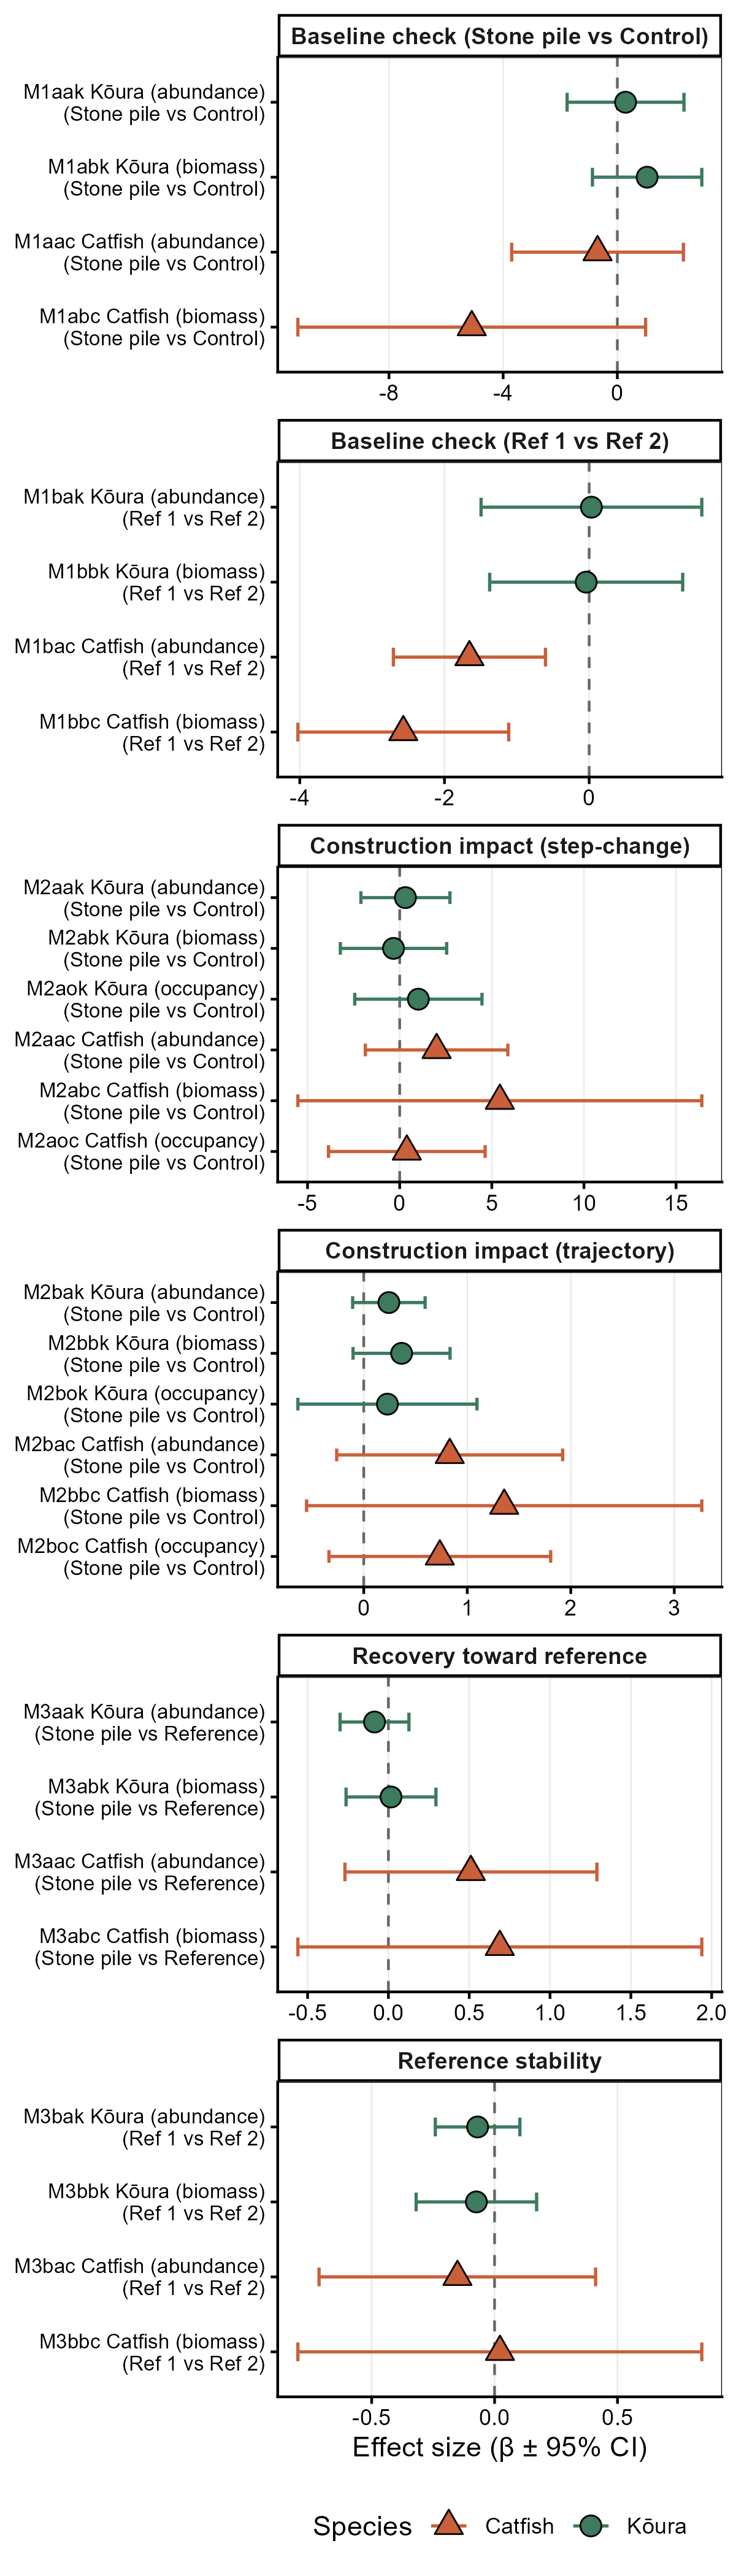
\includegraphics[width=3in,height=\textheight,keepaspectratio]{outputs/fig-forest-plot.png}

}

\caption{\label{fig-forest-plot}Effect sizes (\(\beta\) ± 95\% CI) for
the key term of interest of every model in model\_registry (kōura and
catfish, RQ1--RQ4). Filled points indicate significant effects (p
\textless{} 0.05). Each panel has its own x-axis scale --- \(\beta\)
magnitudes are not directly comparable across panels because each RQ
tests a different contrast (step-change, per-round slope, or simple
group difference) and RQ1 occupancy is on the log-odds scale while all
others use the Tweedie log link. Models with degenerate confidence
intervals (non-positive-definite Hessian) are excluded.}

\end{figure}%

\begin{figure}

\centering{


\includegraphics[width=5in,height=\textheight,keepaspectratio]{outputs/fig-koura-trends.png}

}

\caption{\label{fig-koura-trends}Mean catch per monitoring round (± 95\%
CI) by site type for kōura.}

\end{figure}%

\begin{figure}

\centering{

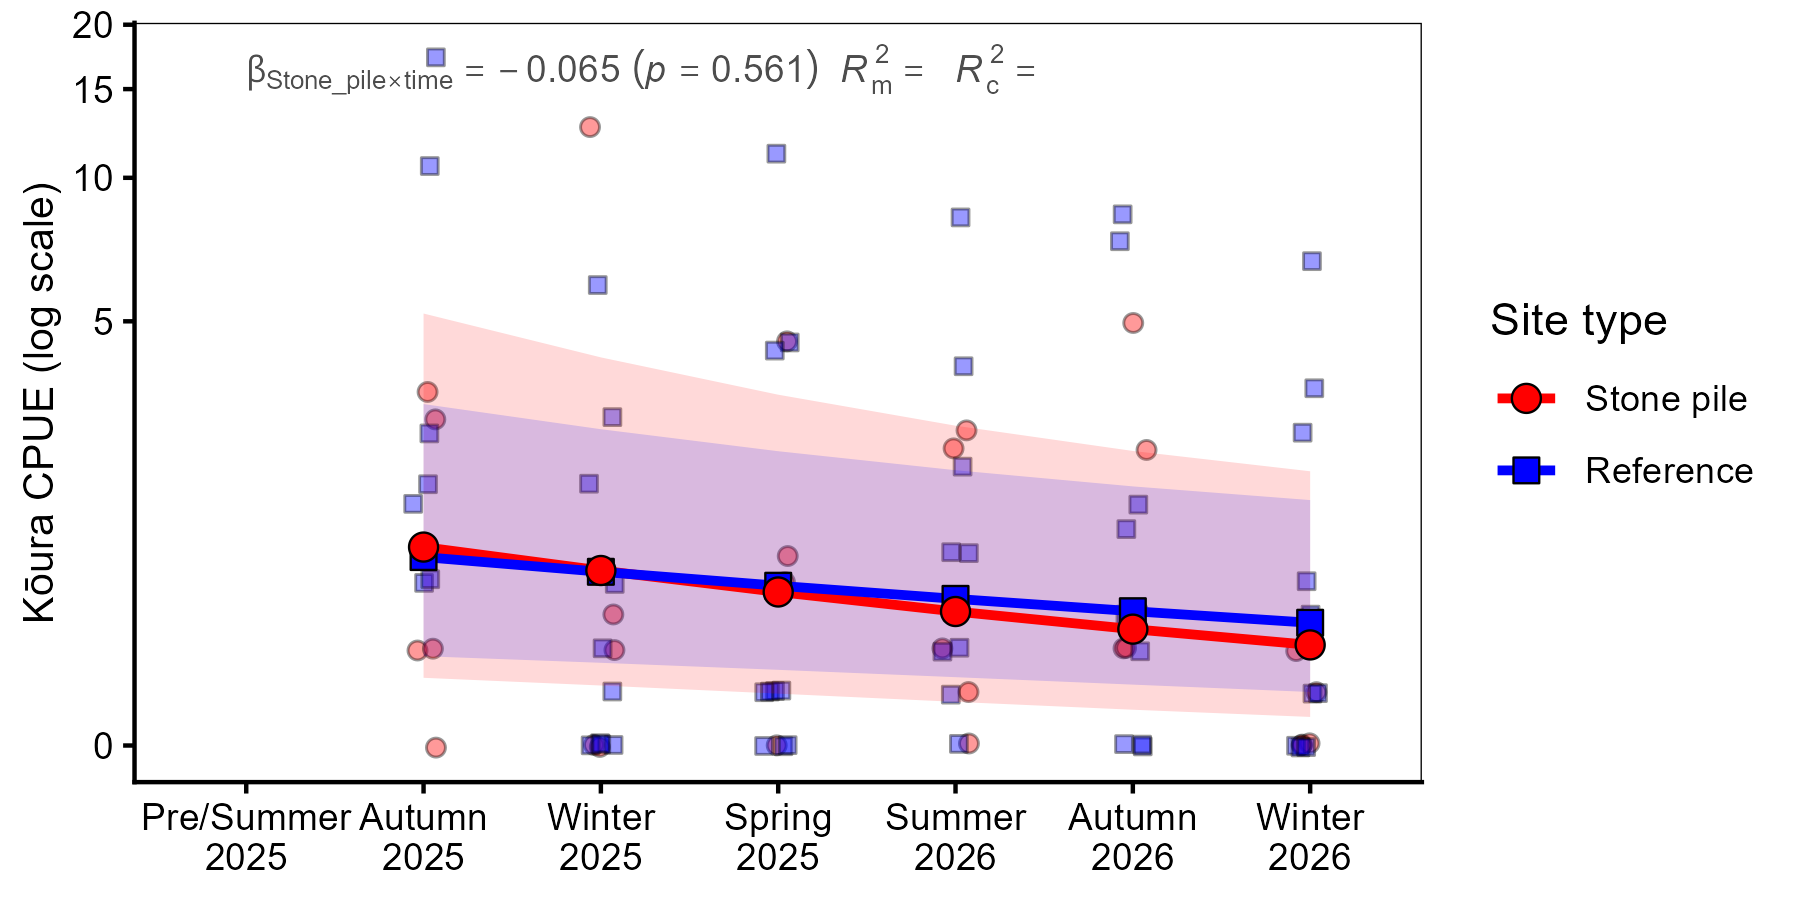
\includegraphics[width=6.5in,height=\textheight,keepaspectratio]{outputs/fig-convergence-plot.png}

}

\caption{\label{fig-convergence-plot}Predicted kōura CPUE trajectories
over monitoring rounds at stone pile and reference sites from the
abundance convergence model. Shaded ribbons represent 95\% confidence
intervals. The annotation shows the key interaction term (\(\beta\) ±
p-value) and model R² values for fixed effects (R²m) and conditional
(R²c).}

\end{figure}%

\begin{figure}

\centering{

\pandocbounded{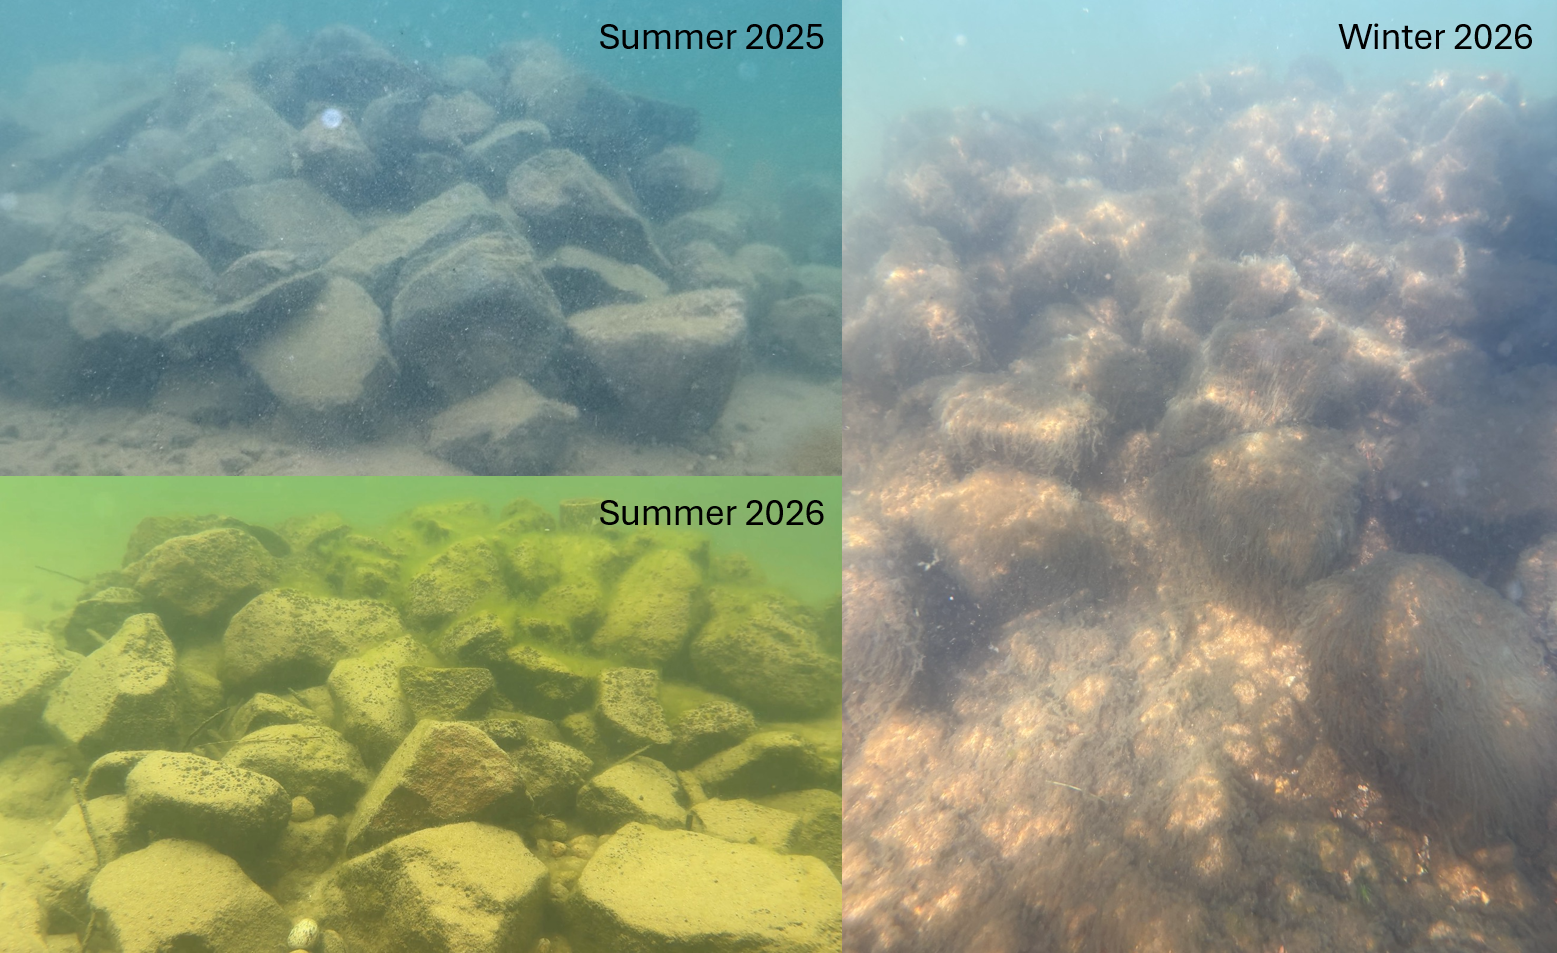
\includegraphics[keepaspectratio]{images/Stone_pile_devalopment.png}}

}

\caption{\label{fig-stone-piles}Progressive algal biofouling at stone
pile site 9 in Lake Rotoiti across three monitoring periods. Summer 2025
(top left, shortly after construction) shows clean stone surfaces with
open interstitial spaces. By Summer 2026 (bottom left) moderate biofilm
accumulation is visible. Winter 2026 (right) shows complete cover of
stone surfaces by filamentous algae.}

\end{figure}%

\subsection{Supplementary information}\label{supplementary-information}

\emph{Supplementary figures are provided in the appendices.}

\begin{longtable}[]{@{}
  >{\raggedright\arraybackslash}p{(\linewidth - 26\tabcolsep) * \real{0.0536}}
  >{\raggedright\arraybackslash}p{(\linewidth - 26\tabcolsep) * \real{0.0298}}
  >{\raggedright\arraybackslash}p{(\linewidth - 26\tabcolsep) * \real{0.0476}}
  >{\raggedright\arraybackslash}p{(\linewidth - 26\tabcolsep) * \real{0.0833}}
  >{\raggedright\arraybackslash}p{(\linewidth - 26\tabcolsep) * \real{0.0774}}
  >{\raggedright\arraybackslash}p{(\linewidth - 26\tabcolsep) * \real{0.0655}}
  >{\raggedright\arraybackslash}p{(\linewidth - 26\tabcolsep) * \real{0.2560}}
  >{\raggedleft\arraybackslash}p{(\linewidth - 26\tabcolsep) * \real{0.0536}}
  >{\raggedleft\arraybackslash}p{(\linewidth - 26\tabcolsep) * \real{0.0595}}
  >{\raggedleft\arraybackslash}p{(\linewidth - 26\tabcolsep) * \real{0.0595}}
  >{\raggedleft\arraybackslash}p{(\linewidth - 26\tabcolsep) * \real{0.0476}}
  >{\raggedleft\arraybackslash}p{(\linewidth - 26\tabcolsep) * \real{0.0536}}
  >{\raggedleft\arraybackslash}p{(\linewidth - 26\tabcolsep) * \real{0.0536}}
  >{\raggedleft\arraybackslash}p{(\linewidth - 26\tabcolsep) * \real{0.0595}}@{}}
\caption{Full fixed-effect estimates (β, SE, 95\% CI, p-value) for every
term in every model currently in model\_registry. Unlike the
interaction-only summary above, this surfaces covariate effects
(e.g.~Substrate\_index\_after, Season) directly rather than requiring a
one-off check per model.}\tabularnewline
\toprule\noalign{}
\begin{minipage}[b]{\linewidth}\raggedright
model\_id
\end{minipage} & \begin{minipage}[b]{\linewidth}\raggedright
RQ
\end{minipage} & \begin{minipage}[b]{\linewidth}\raggedright
species
\end{minipage} & \begin{minipage}[b]{\linewidth}\raggedright
response\_type
\end{minipage} & \begin{minipage}[b]{\linewidth}\raggedright
comparison
\end{minipage} & \begin{minipage}[b]{\linewidth}\raggedright
time\_frame
\end{minipage} & \begin{minipage}[b]{\linewidth}\raggedright
term
\end{minipage} & \begin{minipage}[b]{\linewidth}\raggedleft
estimate
\end{minipage} & \begin{minipage}[b]{\linewidth}\raggedleft
std.error
\end{minipage} & \begin{minipage}[b]{\linewidth}\raggedleft
statistic
\end{minipage} & \begin{minipage}[b]{\linewidth}\raggedleft
p.value
\end{minipage} & \begin{minipage}[b]{\linewidth}\raggedleft
p\_adj\_BH
\end{minipage} & \begin{minipage}[b]{\linewidth}\raggedleft
conf.low
\end{minipage} & \begin{minipage}[b]{\linewidth}\raggedleft
conf.high
\end{minipage} \\
\midrule\noalign{}
\endfirsthead
\toprule\noalign{}
\begin{minipage}[b]{\linewidth}\raggedright
model\_id
\end{minipage} & \begin{minipage}[b]{\linewidth}\raggedright
RQ
\end{minipage} & \begin{minipage}[b]{\linewidth}\raggedright
species
\end{minipage} & \begin{minipage}[b]{\linewidth}\raggedright
response\_type
\end{minipage} & \begin{minipage}[b]{\linewidth}\raggedright
comparison
\end{minipage} & \begin{minipage}[b]{\linewidth}\raggedright
time\_frame
\end{minipage} & \begin{minipage}[b]{\linewidth}\raggedright
term
\end{minipage} & \begin{minipage}[b]{\linewidth}\raggedleft
estimate
\end{minipage} & \begin{minipage}[b]{\linewidth}\raggedleft
std.error
\end{minipage} & \begin{minipage}[b]{\linewidth}\raggedleft
statistic
\end{minipage} & \begin{minipage}[b]{\linewidth}\raggedleft
p.value
\end{minipage} & \begin{minipage}[b]{\linewidth}\raggedleft
p\_adj\_BH
\end{minipage} & \begin{minipage}[b]{\linewidth}\raggedleft
conf.low
\end{minipage} & \begin{minipage}[b]{\linewidth}\raggedleft
conf.high
\end{minipage} \\
\midrule\noalign{}
\endhead
\bottomrule\noalign{}
\endlastfoot
M1aac & RQ1 & Catfish & abundance & treatment & before & (Intercept) &
-2.303 & 0.908 & -2.535 & 0.011 & NA & -4.083 & -0.522 \\
M1aac & RQ1 & Catfish & abundance & treatment & before &
Site\_type\_detailStone\_pile & -0.693 & 1.535 & -0.452 & 0.652 & 0.783
& -3.701 & 2.315 \\
M1abc & RQ1 & Catfish & biomass & treatment & before & (Intercept) &
3.203 & 1.279 & 2.504 & 0.012 & NA & 0.696 & 5.709 \\
M1abc & RQ1 & Catfish & biomass & treatment & before &
Site\_type\_detailStone\_pile & -5.100 & 3.107 & -1.641 & 0.101 & 0.403
& -11.190 & 0.990 \\
M1aak & RQ1 & Kōura & abundance & treatment & before & (Intercept) &
-1.897 & 0.785 & -2.415 & 0.016 & NA & -3.437 & -0.358 \\
M1aak & RQ1 & Kōura & abundance & treatment & before &
Site\_type\_detailStone\_pile & 0.288 & 1.044 & 0.276 & 0.783 & 0.783 &
-1.759 & 2.334 \\
M1abk & RQ1 & Kōura & biomass & treatment & before & (Intercept) & 1.030
& 0.830 & 1.241 & 0.215 & NA & -0.597 & 2.656 \\
M1abk & RQ1 & Kōura & biomass & treatment & before &
Site\_type\_detailStone\_pile & 1.044 & 0.977 & 1.068 & 0.286 & 0.571 &
-0.872 & 2.959 \\
M1bac & RQ1 & Catfish & abundance & reference & before & (Intercept) &
-102.299 & 32.656 & -3.133 & 0.002 & NA & -166.303 & -38.295 \\
M1bac & RQ1 & Catfish & abundance & reference & before &
Site\_type\_detailReference\_2 & -1.655 & 0.536 & -3.087 & 0.002 & 0.004
& -2.706 & -0.604 \\
M1bac & RQ1 & Catfish & abundance & reference & before & Temperature &
4.079 & 1.293 & 3.154 & 0.002 & NA & 1.544 & 6.613 \\
M1bbc & RQ1 & Catfish & biomass & reference & before & (Intercept) &
-153.136 & 37.363 & -4.099 & 0.000 & NA & -226.366 & -79.906 \\
M1bbc & RQ1 & Catfish & biomass & reference & before &
Site\_type\_detailReference\_2 & -2.569 & 0.743 & -3.457 & 0.001 & 0.002
& -4.026 & -1.112 \\
M1bbc & RQ1 & Catfish & biomass & reference & before & Temperature &
6.315 & 1.482 & 4.261 & 0.000 & NA & 3.410 & 9.220 \\
M1bak & RQ1 & Kōura & abundance & reference & before & (Intercept) &
0.742 & 0.553 & 1.343 & 0.179 & NA & -0.341 & 1.825 \\
M1bak & RQ1 & Kōura & abundance & reference & before &
Site\_type\_detailReference\_2 & 0.031 & 0.778 & 0.040 & 0.968 & 0.968 &
-1.494 & 1.557 \\
M1bbk & RQ1 & Kōura & biomass & reference & before & (Intercept) & 3.623
& 0.478 & 7.580 & 0.000 & NA & 2.686 & 4.560 \\
M1bbk & RQ1 & Kōura & biomass & reference & before &
Site\_type\_detailReference\_2 & -0.041 & 0.681 & -0.061 & 0.952 & 0.968
& -1.375 & 1.293 \\
M2aac & RQ2a & Catfish & abundance & vs\_control & full & (Intercept) &
-3.777 & 1.721 & -2.196 & 0.028 & NA & -7.150 & -0.405 \\
M2aac & RQ2a & Catfish & abundance & vs\_control & full & PeriodAfter &
0.664 & 1.505 & 0.442 & 0.659 & NA & -2.285 & 3.613 \\
M2aac & RQ2a & Catfish & abundance & vs\_control & full &
siteStone\_pile & -0.694 & 1.752 & -0.396 & 0.692 & NA & -4.127 &
2.738 \\
M2aac & RQ2a & Catfish & abundance & vs\_control & full &
monitoring\_int & -0.291 & 0.336 & -0.868 & 0.385 & NA & -0.949 &
0.367 \\
M2aac & RQ2a & Catfish & abundance & vs\_control & full &
PeriodAfter:siteStone\_pile & 2.007 & 1.956 & 1.026 & 0.305 & 0.861 &
-1.828 & 5.842 \\
M2abc & RQ2a & Catfish & biomass & vs\_control & full & (Intercept) &
1.770 & 2.734 & 0.647 & 0.517 & NA & -3.589 & 7.128 \\
M2abc & RQ2a & Catfish & biomass & vs\_control & full & PeriodAfter &
-0.330 & 2.264 & -0.146 & 0.884 & NA & -4.767 & 4.107 \\
M2abc & RQ2a & Catfish & biomass & vs\_control & full & siteStone\_pile
& -5.279 & 5.667 & -0.932 & 0.352 & NA & -16.386 & 5.827 \\
M2abc & RQ2a & Catfish & biomass & vs\_control & full & monitoring\_int
& -0.354 & 0.483 & -0.731 & 0.465 & NA & -1.301 & 0.594 \\
M2abc & RQ2a & Catfish & biomass & vs\_control & full &
PeriodAfter:siteStone\_pile & 5.309 & 5.572 & 0.953 & 0.341 & 0.861 &
-5.611 & 16.229 \\
M2aoc & RQ2a & Catfish & occupancy & vs\_control & full & (Intercept) &
-2.029 & 1.853 & -1.095 & 0.274 & NA & -5.661 & 1.604 \\
M2aoc & RQ2a & Catfish & occupancy & vs\_control & full & PeriodAfter &
-0.148 & 1.734 & -0.085 & 0.932 & NA & -3.548 & 3.251 \\
M2aoc & RQ2a & Catfish & occupancy & vs\_control & full &
siteStone\_pile & 0.000 & 1.947 & 0.000 & 1.000 & NA & -3.815 & 3.815 \\
M2aoc & RQ2a & Catfish & occupancy & vs\_control & full &
monitoring\_int & -0.160 & 0.255 & -0.628 & 0.530 & NA & -0.661 &
0.340 \\
M2aoc & RQ2a & Catfish & occupancy & vs\_control & full &
PeriodAfter:siteStone\_pile & 0.374 & 2.132 & 0.175 & 0.861 & 0.861 &
-3.805 & 4.552 \\
M2aak & RQ2a & Kōura & abundance & vs\_control & full & (Intercept) &
-2.753 & 1.183 & -2.327 & 0.020 & NA & -5.072 & -0.434 \\
M2aak & RQ2a & Kōura & abundance & vs\_control & full & PeriodAfter &
2.374 & 0.976 & 2.432 & 0.015 & NA & 0.461 & 4.286 \\
M2aak & RQ2a & Kōura & abundance & vs\_control & full & siteStone\_pile
& 0.751 & 1.335 & 0.563 & 0.574 & NA & -1.865 & 3.368 \\
M2aak & RQ2a & Kōura & abundance & vs\_control & full & monitoring\_int
& -0.253 & 0.082 & -3.094 & 0.002 & NA & -0.413 & -0.093 \\
M2aak & RQ2a & Kōura & abundance & vs\_control & full &
PeriodAfter:siteStone\_pile & 0.311 & 1.232 & 0.253 & 0.800 & 0.861 &
-2.104 & 2.727 \\
M2abk & RQ2a & Kōura & biomass & vs\_control & full & (Intercept) &
0.315 & 1.335 & 0.236 & 0.813 & NA & -2.301 & 2.931 \\
M2abk & RQ2a & Kōura & biomass & vs\_control & full & PeriodAfter &
2.248 & 1.246 & 1.805 & 0.071 & NA & -0.193 & 4.689 \\
M2abk & RQ2a & Kōura & biomass & vs\_control & full & siteStone\_pile &
1.410 & 1.552 & 0.909 & 0.363 & NA & -1.631 & 4.451 \\
M2abk & RQ2a & Kōura & biomass & vs\_control & full & monitoring\_int &
-0.196 & 0.110 & -1.791 & 0.073 & NA & -0.412 & 0.019 \\
M2abk & RQ2a & Kōura & biomass & vs\_control & full &
PeriodAfter:siteStone\_pile & -0.336 & 1.471 & -0.228 & 0.819 & 0.861 &
-3.220 & 2.548 \\
M2aok & RQ2a & Kōura & occupancy & vs\_control & full & (Intercept) &
-0.690 & 1.643 & -0.420 & 0.674 & NA & -3.911 & 2.530 \\
M2aok & RQ2a & Kōura & occupancy & vs\_control & full & PeriodAfter &
1.913 & 1.556 & 1.230 & 0.219 & NA & -1.136 & 4.963 \\
M2aok & RQ2a & Kōura & occupancy & vs\_control & full & siteStone\_pile
& 0.013 & 2.121 & 0.006 & 0.995 & NA & -4.144 & 4.171 \\
M2aok & RQ2a & Kōura & occupancy & vs\_control & full & monitoring\_int
& -0.286 & 0.215 & -1.333 & 0.183 & NA & -0.708 & 0.135 \\
M2aok & RQ2a & Kōura & occupancy & vs\_control & full &
PeriodAfter:siteStone\_pile & 1.013 & 1.762 & 0.575 & 0.565 & 0.861 &
-2.440 & 4.466 \\
M2bac & RQ2b & Catfish & abundance & vs\_control & after & (Intercept) &
-1.974 & 1.605 & -1.230 & 0.219 & NA & -5.121 & 1.172 \\
M2bac & RQ2b & Catfish & abundance & vs\_control & after &
siteStone\_pile & -1.425 & 1.826 & -0.781 & 0.435 & NA & -5.004 &
2.153 \\
M2bac & RQ2b & Catfish & abundance & vs\_control & after &
monitoring\_int & -0.633 & 0.407 & -1.556 & 0.120 & NA & -1.430 &
0.164 \\
M2bac & RQ2b & Catfish & abundance & vs\_control & after &
siteStone\_pile:monitoring\_int & 0.828 & 0.555 & 1.491 & 0.136 & 0.224
& -0.260 & 1.916 \\
M2bbc & RQ2b & Catfish & biomass & vs\_control & after & (Intercept) &
3.787 & 1.990 & 1.903 & 0.057 & NA & -0.113 & 7.687 \\
M2bbc & RQ2b & Catfish & biomass & vs\_control & after & siteStone\_pile
& -4.231 & 3.386 & -1.250 & 0.211 & NA & -10.867 & 2.404 \\
M2bbc & RQ2b & Catfish & biomass & vs\_control & after & monitoring\_int
& -0.956 & 0.676 & -1.415 & 0.157 & NA & -2.280 & 0.368 \\
M2bbc & RQ2b & Catfish & biomass & vs\_control & after &
siteStone\_pile:monitoring\_int & 1.323 & 0.941 & 1.407 & 0.159 & 0.224
& -0.520 & 3.167 \\
M2boc & RQ2b & Catfish & occupancy & vs\_control & after & (Intercept) &
-0.819 & 1.663 & -0.493 & 0.622 & NA & -4.080 & 2.441 \\
M2boc & RQ2b & Catfish & occupancy & vs\_control & after &
siteStone\_pile & -1.954 & 1.896 & -1.031 & 0.303 & NA & -5.670 &
1.761 \\
M2boc & RQ2b & Catfish & occupancy & vs\_control & after &
monitoring\_int & -0.545 & 0.412 & -1.324 & 0.185 & NA & -1.352 &
0.262 \\
M2boc & RQ2b & Catfish & occupancy & vs\_control & after &
siteStone\_pile:monitoring\_int & 0.707 & 0.535 & 1.322 & 0.186 & 0.224
& -0.342 & 1.756 \\
M2bak & RQ2b & Kōura & abundance & vs\_control & after & (Intercept) &
0.084 & 0.846 & 0.099 & 0.921 & NA & -1.573 & 1.741 \\
M2bak & RQ2b & Kōura & abundance & vs\_control & after & siteStone\_pile
& 0.323 & 0.808 & 0.400 & 0.689 & NA & -1.261 & 1.907 \\
M2bak & RQ2b & Kōura & abundance & vs\_control & after & monitoring\_int
& -0.409 & 0.143 & -2.861 & 0.004 & NA & -0.690 & -0.129 \\
M2bak & RQ2b & Kōura & abundance & vs\_control & after &
siteStone\_pile:monitoring\_int & 0.243 & 0.179 & 1.359 & 0.174 & 0.224
& -0.107 & 0.593 \\
M2bbk & RQ2b & Kōura & biomass & vs\_control & after & (Intercept) &
3.270 & 0.856 & 3.821 & 0.000 & NA & 1.593 & 4.948 \\
M2bbk & RQ2b & Kōura & biomass & vs\_control & after & siteStone\_pile &
-0.077 & 0.986 & -0.078 & 0.938 & NA & -2.010 & 1.856 \\
M2bbk & RQ2b & Kōura & biomass & vs\_control & after & monitoring\_int &
-0.427 & 0.191 & -2.240 & 0.025 & NA & -0.800 & -0.053 \\
M2bbk & RQ2b & Kōura & biomass & vs\_control & after &
siteStone\_pile:monitoring\_int & 0.366 & 0.239 & 1.531 & 0.126 & 0.224
& -0.103 & 0.834 \\
M2bok & RQ2b & Kōura & occupancy & vs\_control & after & (Intercept) &
1.585 & 1.885 & 0.841 & 0.400 & NA & -2.109 & 5.280 \\
M2bok & RQ2b & Kōura & occupancy & vs\_control & after & siteStone\_pile
& 0.563 & 2.660 & 0.212 & 0.832 & NA & -4.651 & 5.776 \\
M2bok & RQ2b & Kōura & occupancy & vs\_control & after & monitoring\_int
& -0.403 & 0.311 & -1.296 & 0.195 & NA & -1.014 & 0.207 \\
M2bok & RQ2b & Kōura & occupancy & vs\_control & after &
siteStone\_pile:monitoring\_int & 0.229 & 0.441 & 0.519 & 0.604 & 0.604
& -0.636 & 1.094 \\
M3aac & RQ3a & Catfish & abundance & vs\_reference & after & (Intercept)
& -7.151 & 1.282 & -5.577 & 0.000 & NA & -9.664 & -4.638 \\
M3aac & RQ3a & Catfish & abundance & vs\_reference & after &
siteStone\_pile & -2.471 & 1.940 & -1.274 & 0.203 & NA & -6.273 &
1.331 \\
M3aac & RQ3a & Catfish & abundance & vs\_reference & after &
monitoring\_int & -0.215 & 0.147 & -1.462 & 0.144 & NA & -0.504 &
0.073 \\
M3aac & RQ3a & Catfish & abundance & vs\_reference & after & Temperature
& 0.315 & 0.058 & 5.414 & 0.000 & NA & 0.201 & 0.429 \\
M3aac & RQ3a & Catfish & abundance & vs\_reference & after &
siteStone\_pile:monitoring\_int & 0.510 & 0.398 & 1.283 & 0.199 & 0.559
& -0.269 & 1.290 \\
M3abc & RQ3a & Catfish & biomass & vs\_reference & after & (Intercept) &
3.011 & 1.189 & 2.532 & 0.011 & NA & 0.681 & 5.342 \\
M3abc & RQ3a & Catfish & biomass & vs\_reference & after &
siteStone\_pile & -4.370 & 3.059 & -1.429 & 0.153 & NA & -10.366 &
1.626 \\
M3abc & RQ3a & Catfish & biomass & vs\_reference & after &
monitoring\_int & -0.250 & 0.209 & -1.196 & 0.232 & NA & -0.660 &
0.160 \\
M3abc & RQ3a & Catfish & biomass & vs\_reference & after &
siteStone\_pile:monitoring\_int & 0.689 & 0.638 & 1.081 & 0.280 & 0.559
& -0.560 & 1.939 \\
M3aak & RQ3a & Kōura & abundance & vs\_reference & after & (Intercept) &
0.229 & 0.519 & 0.440 & 0.660 & NA & -0.789 & 1.247 \\
M3aak & RQ3a & Kōura & abundance & vs\_reference & after &
siteStone\_pile & 0.217 & 0.901 & 0.240 & 0.810 & NA & -1.550 & 1.984 \\
M3aak & RQ3a & Kōura & abundance & vs\_reference & after &
monitoring\_int & -0.090 & 0.056 & -1.612 & 0.107 & NA & -0.199 &
0.019 \\
M3aak & RQ3a & Kōura & abundance & vs\_reference & after &
siteStone\_pile:monitoring\_int & -0.086 & 0.109 & -0.791 & 0.429 &
0.572 & -0.299 & 0.127 \\
M3abk & RQ3a & Kōura & biomass & vs\_reference & after & (Intercept) &
3.369 & 0.506 & 6.655 & 0.000 & NA & 2.377 & 4.361 \\
M3abk & RQ3a & Kōura & biomass & vs\_reference & after & siteStone\_pile
& -0.149 & 0.885 & -0.168 & 0.866 & NA & -1.884 & 1.586 \\
M3abk & RQ3a & Kōura & biomass & vs\_reference & after & monitoring\_int
& -0.088 & 0.074 & -1.177 & 0.239 & NA & -0.234 & 0.058 \\
M3abk & RQ3a & Kōura & biomass & vs\_reference & after &
siteStone\_pile:monitoring\_int & 0.016 & 0.142 & 0.112 & 0.911 & 0.911
& -0.262 & 0.294 \\
M3bac & RQ3b & Catfish & abundance & reference & after & (Intercept) &
-7.372 & 1.705 & -4.324 & 0.000 & NA & -10.713 & -4.031 \\
M3bac & RQ3b & Catfish & abundance & reference & after &
Site\_type\_detailReference\_2 & 0.753 & 1.007 & 0.747 & 0.455 & NA &
-1.221 & 2.726 \\
M3bac & RQ3b & Catfish & abundance & reference & after & monitoring\_int
& -0.130 & 0.220 & -0.591 & 0.555 & NA & -0.562 & 0.301 \\
M3bac & RQ3b & Catfish & abundance & reference & after & Temperature &
0.304 & 0.073 & 4.183 & 0.000 & NA & 0.161 & 0.446 \\
M3bac & RQ3b & Catfish & abundance & reference & after &
Site\_type\_detailReference\_2:monitoring\_int & -0.151 & 0.287 & -0.527
& 0.598 & 0.797 & -0.714 & 0.411 \\
M3bbc & RQ3b & Catfish & biomass & reference & after & (Intercept) &
2.726 & 1.556 & 1.752 & 0.080 & NA & -0.324 & 5.775 \\
M3bbc & RQ3b & Catfish & biomass & reference & after &
Site\_type\_detailReference\_2 & 0.191 & 1.640 & 0.116 & 0.907 & NA &
-3.024 & 3.406 \\
M3bbc & RQ3b & Catfish & biomass & reference & after & monitoring\_int &
-0.227 & 0.301 & -0.754 & 0.451 & NA & -0.816 & 0.363 \\
M3bbc & RQ3b & Catfish & biomass & reference & after &
Site\_type\_detailReference\_2:monitoring\_int & 0.022 & 0.419 & 0.052 &
0.959 & 0.959 & -0.800 & 0.843 \\
M3bak & RQ3b & Kōura & abundance & reference & after & (Intercept) &
0.380 & 0.790 & 0.480 & 0.631 & NA & -1.169 & 1.928 \\
M3bak & RQ3b & Kōura & abundance & reference & after &
Site\_type\_detailReference\_2 & -0.115 & 0.570 & -0.202 & 0.840 & NA &
-1.232 & 1.002 \\
M3bak & RQ3b & Kōura & abundance & reference & after & monitoring\_int &
-0.019 & 0.062 & -0.302 & 0.763 & NA & -0.141 & 0.103 \\
M3bak & RQ3b & Kōura & abundance & reference & after & SeasonSpring &
-0.386 & 0.227 & -1.699 & 0.089 & NA & -0.831 & 0.059 \\
M3bak & RQ3b & Kōura & abundance & reference & after & SeasonSummer &
-0.330 & 0.233 & -1.416 & 0.157 & NA & -0.787 & 0.127 \\
M3bak & RQ3b & Kōura & abundance & reference & after & SeasonWinter &
-0.546 & 0.196 & -2.781 & 0.005 & NA & -0.932 & -0.161 \\
M3bak & RQ3b & Kōura & abundance & reference & after &
Site\_type\_detailReference\_2:monitoring\_int & -0.069 & 0.088 & -0.787
& 0.431 & 0.797 & -0.241 & 0.103 \\
M3bbk & RQ3b & Kōura & biomass & reference & after & (Intercept) & 3.275
& 0.800 & 4.095 & 0.000 & NA & 1.707 & 4.842 \\
M3bbk & RQ3b & Kōura & biomass & reference & after &
Site\_type\_detailReference\_2 & -0.067 & 0.670 & -0.100 & 0.920 & NA &
-1.379 & 1.245 \\
M3bbk & RQ3b & Kōura & biomass & reference & after & monitoring\_int &
-0.047 & 0.087 & -0.548 & 0.584 & NA & -0.217 & 0.122 \\
M3bbk & RQ3b & Kōura & biomass & reference & after &
Site\_type\_detailReference\_2:monitoring\_int & -0.074 & 0.125 & -0.591
& 0.554 & 0.797 & -0.319 & 0.171 \\
\end{longtable}

\protect\phantomsection\label{refs}
\begin{CSLReferences}{1}{0}
\bibitem[\citeproctext]{ref-Adams2007}
Adams S.B. (2007). Direct and indirect effects of channel catfish
({\emph{Ictalurus punctatus}}) on native crayfishes ({Cambaridae}) in
experimental tanks. \emph{The American Midland Naturalist} \textbf{158},
85--96.
\url{https://doi.org/10.1674/0003-0031(2007)158\%5B85:daieoc\%5D2.0.co;2}

\bibitem[\citeproctext]{ref-Barnes1996}
Barnes G.E. (1996). \emph{The biology and general ecology of the brown
bullhead catfish (\emph{ameiurus nebulosus}) in {Lake Taupo}}.
University of Waikato, Hamilton, New Zealand.

\bibitem[\citeproctext]{ref-Barnes2003}
Barnes G.E. \& Hicks B.J. (2003). Brown bullhead catfish
({\emph{Ameiurus nebulosus}}) in {Lake Taupo}. In: \emph{Managing
invasive freshwater fish in {New Zealand}: Proceedings of a workshop
hosted by {Department of Conservation}, 10-12 may 2001, {Hamilton}}.
Department of Conservation.

\bibitem[\citeproctext]{ref-Bates2015}
Bates D., Mächler M., Bolker B. \& Walker S. (2015). Fitting linear
mixed-effects models using {lme4}. \emph{Journal of Statistical
Software} \textbf{67}, 1--48.
\url{https://doi.org/10.18637/jss.v067.i01}

\bibitem[\citeproctext]{ref-Blanchfield2026}
Blanchfield P.J., Rodrigues T.H., MacNeil C., Stewart S., Lee F., Hicks
B.J., \emph{et al.} (2026). Invadingbrown bullhead catfish (ameiurus
nebulosus) show thermal niche rigidity and benthic niche plasticity:
Implications for management. \emph{Biological Invasions}.
\url{https://doi.org/10.1007/s10530-026-03877-5}

\bibitem[\citeproctext]{ref-Brooks2017}
Brooks M., Bolker B., Kristensen K., Maechler M., Magnusson A., Skaug
H., \emph{et al.} (2017).
\href{https://doi.org/10.32614/cran.package.glmmtmb}{glmmTMB:
Generalized linear mixed models using template model builder}.
\emph{CRAN: Contributed Packages}

\bibitem[\citeproctext]{ref-Burkner2018}
Bürkner P.-C. (2018). Advanced bayesian multilevel modeling with the r
package brms. \emph{The R Journal} \textbf{10}, 395.
\url{https://doi.org/10.32614/rj-2018-017}

\bibitem[\citeproctext]{ref-Burkner2017}
Bürkner P.-C. (2017).
\textless B\textgreater brms\textless/b\textgreater{} : An
\textless i\textgreater r\textless/i\textgreater{} package for bayesian
multilevel models using
\textless i\textgreater stan\textless/i\textgreater. \emph{Journal of
Statistical Software} \textbf{80}.
\url{https://doi.org/10.18637/jss.v080.i01}

\bibitem[\citeproctext]{ref-Burnham2002}
Burnham K.P. \& R. A.D. (2002).
\href{https://doi.org/10.1007/978-0-387-22456-5_6}{Advanced issues and
deeper insights}. In: \emph{Model selection and multimodel inference: A
practical information-theoretic approach}. pp. 267--351. Springer, New
York, NY.

\bibitem[\citeproctext]{ref-Collier1997}
Collier K.J., Parkyn S.M. \& Rabeni C.F. (1997). Koura: A keystone
species. \emph{Water and Atmosphere} \textbf{5}, 18--20

\bibitem[\citeproctext]{ref-Dedual2002}
Dedual M. (2002). Vertical distribution and movements of brown bullhead
({\emph{Ameiurus nebulosus}} {Lesueur} 1819) in {Motuoapa Bay}, southern
{Lake Taupo}, {New Zealand}. \emph{Hydrobiologia} \textbf{483},
129--135. \url{https://doi.org/10.1007/978-94-017-0771-8_15}

\bibitem[\citeproctext]{ref-Devcich1979}
Devcich A.A. (1979). \emph{An ecological study of {\emph{Paranephrops
planifrons}} {White} ({Decapoda} : {Parastacidae}) in {Lake Rotoiti},
{North Island}}. University of Waikato, Hamilton, New Zealand.

\bibitem[\citeproctext]{ref-Francis2019}
Francis L.B. (2019).
\emph{\href{https://researchcommons.waikato.ac.nz/handle/10289/12746}{Evaluating
the effects of invasive brown bullhead catfish ({\emph{Ameiurus
nebulosus}}) on k{ō}ura (freshwater crayfish, {\emph{Paranephrops
planifrons}}) in {Lake Rotoiti}}}. University of Waikato.

\bibitem[\citeproctext]{ref-Froese2006}
Froese R. (2006). Cube law, condition factor and weight-length
relationships: History, meta-analysis and recommendations. \emph{Journal
of Applied Ichthyology} \textbf{22}, 241--253.
\url{https://doi.org/10.1111/j.1439-0426.2006.00805.x}

\bibitem[\citeproctext]{ref-Gabry2025}
Gabry J., Češnovar R., Johnson A. \& Bronder S. (2025).
\emph{\href{https://mc-stan.org/cmdstanr/}{Cmdstanr: R interface to
'CmdStan'}}.

\bibitem[\citeproctext]{ref-Grayling2020}
Grayling S. (2020).
\emph{\href{https://atlas.boprc.govt.nz/api/v1/edms/document/A3651696/content}{{Bay
of Plenty} regional pest management plan 2011-2016 annual report for
2019/2020}}. Bay of Plenty Regional Council.

\bibitem[\citeproctext]{ref-Hamilton2005}
Hamilton D., McBride C. \& Uraoka T. (2005). \emph{{Lake Rotoiti}
fieldwork and modelling to support considerations of {Ohau} channel
diversion from {Lake Rotoiti}}. NIWA \& University of Waikato.

\bibitem[\citeproctext]{ref-Hartig2016}
Hartig F. (2016).
\href{https://doi.org/10.32614/cran.package.dharma}{{DHARMa}: Residual
diagnostics for hierarchical (multi-level / mixed) regression models}.
\emph{CRAN: Contributed Packages}

\bibitem[\citeproctext]{ref-Huolila1997}
Huolila M., Marjomäki T.J. \& Laukkanen E. (1997). The success of
crayfish stocking in a dredged river with and without artificial shelter
increase. \emph{Fisheries Research} \textbf{32}, 185--189.
\url{https://doi.org/10.1016/s0165-7836(97)00046-5}

\bibitem[\citeproctext]{ref-Johnsen2008}
Johnsen S.I. \& Taugbøl T. (2008). Add stones, get crayfish -- is it
that simple? \emph{Freshwater Crayfish} \textbf{16}, 47--50

\bibitem[\citeproctext]{ref-Jowett2008}
Jowett I.G., Parkyn S.M. \& Richardson J. (2008). Habitat
characteristics of crayfish ({\emph{Paranephrops planifrons}}) in {New
Zealand} streams using generalised additive models ({GAMs}).
\emph{Hydrobiologia} \textbf{596}, 353--365.
\url{https://doi.org/10.1007/s10750-007-9108-z}

\bibitem[\citeproctext]{ref-Jowett1990}
Jowett I.G. \& Richardson J. (1990). Microhabitat preferences of benthic
invertebrates in a {New Zealand} river and the development of in-stream
flow-habitat models for {\emph{Deleatidium}} spp. \emph{New Zealand
Journal of Marine and Freshwater Research} \textbf{24}, 19--30.
\url{https://doi.org/10.1080/00288330.1990.9516399}

\bibitem[\citeproctext]{ref-Kusabs2023}
Kusabs I.A. (2023). \emph{{Lake Rotorua} alum dosing monitoring
programme 2023 koura and kakahi}. Kusabs \& Associates Ltd, Rotorua, New
Zealand.

\bibitem[\citeproctext]{ref-Kusabs2015a}
Kusabs I.A., Hicks B.J., Quinn J.M. \& Hamilton D.P. (2015a).
Sustainable management of freshwater crayfish (kōura,
{\emph{Paranephrops planifrons}}) in {Te Arawa} ({Rotorua}) lakes,
{North Island}, {New Zealand}. \emph{Fisheries Research} \textbf{168},
35--46. \url{https://doi.org/10.1016/j.fishres.2015.03.015}

\bibitem[\citeproctext]{ref-Kusabs2026}
Kusabs I.A.K., Duggan I.C., Bruere A.C., Scholes P., Te Kurapa T.W.,
Grant T.M., \emph{et al.} (2026). Invasive catfish linked to the decline
of freshwater crayfish in two {Aotearoa New Zealand} lakes.
\emph{Biological Invasions} \textbf{28}.
\url{https://doi.org/10.1007/s10530-026-03852-0}

\bibitem[\citeproctext]{ref-Kusabs2009}
Kusabs I.A. \& Quinn J.M. (2009). Use of a traditional {Māori}
harvesting method, the tau k{ō}ura, for monitoring k{ō}ura (freshwater
crayfish, {\emph{Paranephrops planifrons}}) in {Lake Rotoiti}, {North
Island, New Zealand}. \emph{New Zealand Journal of Marine and Freshwater
Research} \textbf{43}, 713--722.
\url{https://doi.org/10.1080/00288330909510036}

\bibitem[\citeproctext]{ref-Kusabs2015b}
Kusabs I.A., Quinn J.M. \& Hamilton D.P. (2015b). Effects of benthic
substrate, nutrient enrichment and predatory fish on freshwater crayfish
(koura, {\emph{Paranephrops planifrons}}) population characteristics in
seven {Te Arawa} ({Rotorua}) lakes, {North Island}, {New Zealand}.
\emph{Marine and Freshwater Research} \textbf{66}, 631--643.
\url{https://doi.org/10.1071/mf14148}

\bibitem[\citeproctext]{ref-Lee2025}
Lee F., Kusabs I.A.K., Perry G.L.W. \& MacNeil C. (2025). Identifying
refugia from the synergistic threats of climate change and invasive
species. \emph{Web Ecology} \textbf{25}, 221--239.
\url{https://doi.org/10.5194/we-25-221-2025}

\bibitem[\citeproctext]{ref-Lenth2017}
Lenth R.V. \& Piaskowski J. (2017).
\href{https://doi.org/10.32614/cran.package.emmeans}{Emmeans: Estimated
marginal means, aka least-squares means}. \emph{CRAN: Contributed
Packages}

\bibitem[\citeproctext]{ref-MacNeil2025}
MacNeil C., Lee F., Kusabs I. \& Holmes R. (2025). The biter bit;
scavenging behaviour of native freshwater crayfish on the carrion of
native and introduced fish predators in {Aotearoa-New Zealand}.
\emph{Knowledge \& Management of Aquatic Ecosystems}, 29.
\url{https://doi.org/10.1051/kmae/2025022}

\bibitem[\citeproctext]{ref-McDowall1994}
McDowall R.M. (1994). \emph{Gamekeepers for the nation: The story of
{New Zealand}'s {Acclimatisation Society} 1861--1990}. Canterbury
University Press, Christchurch, New Zealand.

\bibitem[\citeproctext]{ref-Momot1995}
Momot W.T. (1995). Redefining the role of crayfish in aquatic
ecosystems. \emph{Reviews in Fisheries Science} \textbf{3}, 33--63.
\url{https://doi.org/10.1080/10641269509388566}

\bibitem[\citeproctext]{ref-Nystrom2006}
Nyström P., Stenroth P., Holmqvist N., Berglund O., Larsson P. \&
Granéli W. (2006). Crayfish in lakes and streams: Individual and
population responses to predation, productivity and substratum
availability. \emph{Freshwater Biology} \textbf{51}, 2096--2113.
\url{https://doi.org/10.1111/j.1365-2427.2006.01641.x}

\bibitem[\citeproctext]{ref-Parkyn2004}
Parkyn S.M. \& Collier K.J. (2004). Interaction of {Press} and {Pulse}
disturbance on crayfish populations: Flood impacts in pasture and forest
streams. \emph{Hydrobiologia} \textbf{527}, 113--124.
\url{https://doi.org/10.1023/b:hydr.0000043189.91134.94}

\bibitem[\citeproctext]{ref-Parkyn2001}
Parkyn S.M., Collier K.J. \& Hicks B.J. (2001). {New Zealand} stream
crayfish: Functional omnivores but trophic predators? \emph{Freshwater
Biology} \textbf{46}, 641--652.
\url{https://doi.org/10.1046/j.1365-2427.2001.00702.x}

\bibitem[\citeproctext]{ref-Parkyn2009}
Parkyn S.M., Meleason M.A. \& Davies-Colley R.J. (2009). Wood enhances
crayfish ({\emph{Paranephrops planifrons}}) habitat in a forested
stream. \emph{New Zealand Journal of Marine and Freshwater Research}
\textbf{43}, 689--700. \url{https://doi.org/10.1080/00288330909510034}

\bibitem[\citeproctext]{ref-Preisser2005}
Preisser E.L., Bolnick D.I. \& Benard M.F. (2005). Scared to death? The
effects of intimidation and consumption in predator-prey interactions.
\emph{Ecology} \textbf{86}, 501--509.
\url{https://doi.org/10.1890/04-0719}

\bibitem[\citeproctext]{ref-Prentice2024}
Prentice M. \& Özkundakci D. (2024).
\emph{\href{https://doi.org/10.15663/eri.report.169}{{Ōhau Channel}
diversion wall: 7-year review: Water quality review and modelling}}. The
University of Waikato.

\bibitem[\citeproctext]{ref-Quinn2002}
Quinn G.P. \& Keough M.J. (2002). \emph{Experimental design and data
analysis for biologists}. Cambridge University Press.

\bibitem[\citeproctext]{ref-RCoreTeam2025}
R Core Team (2025). \emph{\href{https://www.R-project.org/}{{R}: A
language and environment for statistical computing}}. R Foundation for
Statistical Computing, Vienna, Austria.

\bibitem[\citeproctext]{ref-Raven2026b}
Raven O.V., Burdon F.J., Kusabs I.A.K., Holmes R. \& Özkundakci D.
(2026b). Littoral habitat structure influences freshwater crayfish
populations in five volcanic lakes of aotearoa new zealand.
\emph{Hydrobiologia}. \url{https://doi.org/10.1007/s10750-026-06302-z}

\bibitem[\citeproctext]{ref-Raveninreview}
Raven O.V., Holmes R., Kusabs I.A.K., Burdon F.J. \& Özkundakci D. (in
review). \href{https://olivierraven.github.io/Koura_Mesocosm/}{The
importance of structure: Mesocosm evidence for shelter design in
freshwater crayfish restoration}

\bibitem[\citeproctext]{ref-Raven2026a}
Raven O.V., MacNeil C., Lee F., Holmes R., Kusabs I.A.K., Burdon F.J.,
\emph{et al.} (2026a). Fear of the new: A predatory invader provokes
stronger non-consumptive effects on a keystone native prey than a native
predator. \url{https://doi.org/10.21203/rs.3.rs-9891519/v1}

\bibitem[\citeproctext]{ref-Richman2015}
Richman N.I., Böhm M., Adams S.B., Alvarez F., Bergey E.A., Bunn J.J.S.,
\emph{et al.} (2015). Multiple drivers of decline in the global status
of freshwater crayfish ({Decapoda}: {Astacidea}). \emph{Philosophical
Transactions of the Royal Society B: Biological Sciences} \textbf{370},
20140060. \url{https://doi.org/10.1098/rstb.2014.0060}

\bibitem[\citeproctext]{ref-Sayer2025}
Sayer C.A., Fernando E., Jimenez R.R., Macfarlane N.B.W., Rapacciuolo
G., Böhm M., \emph{et al.} (2025). One-quarter of freshwater fauna
threatened with extinction. \emph{Nature} \textbf{638}, 138--145.
\url{https://doi.org/10.1038/s41586-024-08375-z}

\bibitem[\citeproctext]{ref-Scott1973}
Scott W.B. \& Crossman E.J. (1973). \emph{Freshwater fishes of
{Canada}}. Fisheries Research Board of Canada, Ottawa, Canada.

\bibitem[\citeproctext]{ref-Selwood2020}
Selwood K.E. \& Zimmer H.C. (2020). Refuges for biodiversity
conservation: A review of the evidence. \emph{Biological Conservation}
\textbf{245}, 108502. \url{https://doi.org/10.1016/j.biocon.2020.108502}

\bibitem[\citeproctext]{ref-Sheriff2020}
Sheriff M.J., Peacor S.D., Hawlena D. \& Thaker M. (2020).
Non‐consumptive predator effects on prey population size: A dearth of
evidence. \emph{Journal of Animal Ecology} \textbf{89}, 1302--1316.
\url{https://doi.org/10.1111/1365-2656.13213}

\bibitem[\citeproctext]{ref-Streissl2002}
Streissl F. \& Hödl W. (2002). Habitat and shelter requirements of the
stone crayfish, {\emph{Austropotamobius torrentium}} schrank.
\emph{Hydrobiologia} \textbf{477}, 195--199.
\url{https://doi.org/10.1023/A:1021094309738}

\bibitem[\citeproctext]{ref-Underwood1994}
Underwood A.J. (1994). On beyond {BACI}: Sampling designs that might
reliably detect environmental disturbances. \emph{Ecological
Applications} \textbf{4}, 3--15. \url{https://doi.org/10.2307/1942110}

\bibitem[\citeproctext]{ref-Usio2000}
Usio N. \& Townsend C.R. (2000). Distribution of the {New Zealand}
crayfish ({\emph{Paranephrops zealandicus}}) in relation to stream
physico-chemistry, predatory fish, and invertebrate prey. \emph{New
Zealand Journal of Marine and Freshwater Research} \textbf{34},
557--567. \url{https://doi.org/10.1080/00288330.2000.9516957}

\bibitem[\citeproctext]{ref-Vehtari2021}
Vehtari A., Gelman A., Simpson D., Carpenter B. \& Bürkner P.-C. (2021).
Rank-normalization, folding, and localization: An improved Rˆ for
assessing convergence of MCMC (with discussion). \emph{Bayesian
Analysis} \textbf{16}. \url{https://doi.org/10.1214/20-ba1221}

\bibitem[\citeproctext]{ref-Verburg2019}
Verburg P. \& Albert A. (2019).
\emph{\href{https://www.waikatoregion.govt.nz/assets/WRC/TR201918.pdf}{{Lake
Taupo} long-term monitoring programme 2017-2018}}. National Institute of
Water \& Atmospheric Research Ltd, Hamilton.

\bibitem[\citeproctext]{ref-Vincent1984}
Vincent W.F., Gibbs M.M. \& Dryden S.J. (1984). Accelerated
eutrophication in a {New Zealand} lake: {Lake Rotoiti}, central {North
Island}. \emph{New Zealand Journal of Marine and Freshwater Research}
\textbf{18}, 431--440.
\url{https://doi.org/10.1080/00288330.1984.9516064}

\bibitem[\citeproctext]{ref-Woolway2021}
Woolway R.I., Sharma S., Weyhenmeyer G.A., Debolskiy A., Golub M.,
Mercado-Bettín D., \emph{et al.} (2021). Phenological shifts in lake
stratification under climate change. \emph{Nature Communications}
\textbf{12}. \url{https://doi.org/10.1038/s41467-021-22657-4}

\bibitem[\citeproctext]{ref-Zhao2024}
Zhao M., Feng G., Wang H., Shen C., Fu Y., Zhang Y., \emph{et al.}
(2024). The influence of shelter type and coverage on crayfish
({\emph{Procambarus clarkii}}) predation by catfish ({\emph{Silurus
asotus}}): A controlled environment study. \emph{Animals} \textbf{14},
1147. \url{https://doi.org/10.3390/ani14081147}

\end{CSLReferences}




\end{document}
